\documentclass[12pt]{article}

\usepackage{amsmath,amssymb,amsthm}
\usepackage{geometry}
\usepackage{hyperref}
\usepackage{tikz}
\usepackage{tikz-cd}
\usepackage{natbib}
\usepackage{booktabs}
\usepackage{array}
\usepackage{setspace}
\usepackage{parskip}

\usetikzlibrary{
  arrows.meta,
  calc,
  positioning,
  decorations.pathmorphing,
  decorations.markings,
  fit,
  backgrounds
}

\geometry{margin=1.2in}
\onehalfspacing
\setlength{\parskip}{0.55em}

\theoremstyle{plain}
\newtheorem{theorem}{Theorem}[section]
\newtheorem{proposition}[theorem]{Proposition}
\newtheorem{lemma}[theorem]{Lemma}
\newtheorem{corollary}[theorem]{Corollary}

\theoremstyle{definition}
\newtheorem{definition}[theorem]{Definition}
\newtheorem{axiom}[theorem]{Axiom}

\theoremstyle{remark}
\newtheorem{remark}[theorem]{Remark}

% ── Spherepop operator macros ──────────────────────────────────────
\newcommand{\Pop}{\mathbf{Pop}}
\newcommand{\Bind}{\mathbf{Bind}}
\newcommand{\Refuse}{\mathbf{Refuse}}
\newcommand{\Collapse}{\mathbf{Collapse}}
\newcommand{\Merge}{\mathbf{Merge}}
\newcommand{\PathCat}{\mathbb{P}(\Omega)}
\newcommand{\rweight}{\rho}
\newcommand{\picommit}{\pi}
\newcommand{\Lagrangian}{\mathcal{L}}
\newcommand{\Acct}{\mathbf{A}}
\newcommand{\ViewCat}{\mathcal{V}}
\newcommand{\KernelFun}{\mathbf{K}}
\newcommand{\ViewFun}{\mathbf{V}}
\DeclareMathOperator{\GLB}{glb}

\title{\textbf{Identity as Event History}\\[0.4em]
\large Irreversibility, Commitment, and the Ontology of Irreversible Processes}
\author{Flyxion}
\date{\today}

\begin{document}
\maketitle
\thispagestyle{empty}

\begin{abstract}
\noindent
Spherepop is a process-oriented formalism in which the identity of an object is
constituted by the irreversible sequence of transformations that produced it
rather than by its present configuration.  This essay develops the framework
through a single sustained argument in two movements, unified by the central
claim that identity as event history is not a primitive but a derived notion:
it is what remains when possibility has been progressively collapsed.

The first movement establishes the formal infrastructure.  Event words and
normal forms provide a canonical symbolic encoding of object identity.  Directed
acyclic event graphs and causal posets capture branching and parallel structure.
A categorical semantics treats histories as functors from causal index
categories, and merge events are characterised as pushout constructions.
Operational semantics, historical complexity measures, the reconstruction
problem, and a stratified family of equivalence relations complete the
treatment.  The first movement culminates in the Necessity Theorem: under
genuine irreversibility, extensional identity fails as a faithful criterion in
both directions, and historical identity is the only consistent alternative.

The second movement reveals the preimage of the first.  Event histories arise
from a deeper dynamical process: the monotone contraction of a space of
possibilities.  The Spherepop state at any stage is a pair $(\Omega_t, H_t)$
of a shrinking option space and a growing commitment history.  The event word
is the image of the history projection $\Pi_{\mathrm{hist}}$ applied to this
deeper dynamics, making identity a quotient of an irreversible process rather
than a primitive object.  Entropy is derived directly from the geometry of
option-space contraction.  Operators are reinterpreted as typed generators of
event words, classifying the four fundamental modes of exclusion.  Responsibility
weights measure the provenance of each contraction, running as a parallel scalar
beside the entropy measure.

The two movements are unified by a categorical diagram relating the trajectory
category $\mathcal{T}$, the Free History Category $\PathCat$, and the
category of observable states $\mathcal{S}$, with projections $\Pi_{\mathrm{hist}}$
and $\Collapse$ connecting the three levels and neither admitting a right
inverse.  The Worldhood Theorem characterises when a system genuinely inhabits
this structure---when it performs irreversible commitments for which it bears
non-zero responsibility---as opposed to simulating it from a fixed option space.
A discrete variational principle then provides the generative law: realised
trajectories extremize an action functional that balances entropy, responsibility,
and coherence, giving the history of an object the status of an optimal
trajectory, not merely a recorded one.  The essay concludes by placing this
framework in contrast with the set-theoretic ontology it replaces: from
membership to commitment, from static equivalence to irreversible construction,
from objects defined by their contents to processes defined by what they have
made impossible.
\end{abstract}

\vspace{0.8em}
\tableofcontents
\newpage
\section{Introduction}
\label{sec:introduction}

A recurring question in the foundations of mathematics and formal ontology
concerns the correct criterion of identity for objects that exist within
processes rather than in isolation.  Classical set theory locates identity in
the membership relation: two sets are equal precisely when they contain exactly
the same elements, irrespective of how those sets came to exist or in what
order their elements were assembled.  This extensional criterion is powerful
and convenient, but it discards what may be the most significant feature of
many objects encountered in physics, computation, and the theory of complex
systems: that an object's identity is inseparable from the history that
generated it.

Spherepop is a formalism developed to address this gap directly.  Its central
claim is that objects should be represented not as static containers but as
records of transformations, and that identity should be adjudicated by comparing
those records rather than by comparing present states.  The formalism takes
irreversibility as its organising principle.  Because the transformations that
produce objects cannot in general be undone, the historical record accumulates
monotonically; each new event appends to a trace that cannot be retracted.  Two
objects are identical in the Spherepop sense if and only if they are the products
of identical histories.

This essay develops the framework through a single sustained argument in two
interlocking movements, unified by the insight that identity as event history is
not primitive but derived: it is what remains when possibility has been
progressively collapsed.

The first movement takes identity as event history as its immediate object of
study.  It establishes the canonical symbolic encoding of object identity through
event words and normal forms, develops the directed acyclic graph and causal
poset representations of branching histories, provides a categorical semantics
in which histories are functors from causal index categories, characterises merge
events as pushout constructions, analyses operational semantics, historical
complexity measures, and the reconstruction problem, and situates the framework
within the theory of free traced monoidal categories and provenance systems.
The culminating formal result of this movement is the Necessity Theorem
(Section~\ref{sec:necessity}): under conditions of genuine irreversibility,
extensional identity fails as a faithful criterion in both directions, and
historical identity is the only consistent alternative.  This is not the claim
that historical identity is richer or more expressive---which is obvious---but
the stronger claim that extensional identity is positively inadequate: it
conflates objects that are genuinely distinct and fails to cohere with the
structure that irreversibility imposes.

The second movement reveals the preimage of the first.  It asks: what is the
structure from which event histories arise?  The answer is that an event history
is not primitive but is the irreversible boundary trace of a deeper process: the
monotone contraction of a space of possibilities.  A Spherepop object in the
process of being formed is a state pair $(\Omega_t, H_t)$ consisting of what has
already been irrevocably committed and what still remains possible.  The option
space $\Omega_t$ shrinks as the commitment history $H_t$ grows, and the event
word that the first movement treats as primary is the image of the history
projection $\Pi_{\mathrm{hist}}$ applied to this deeper dynamics.  This
reinterpretation makes identity a quotient of an irreversible process: two
objects are identical when their trajectories through possibility space produce
the same ordered boundary trace, regardless of how their option spaces evolved
internally along the way.

The correct relationship between the two movements is vertical, not lateral.
The second does not extend the first by appending new content; it deepens the
first by revealing what the first presupposes.  Identity as event history is the
result of projecting the possibility-history dynamics onto its history coordinate.
Every formal structure in the first movement has a counterpart at this deeper
level, and once the connection is established the two movements read as one: what
identity is, and how identity comes into existence at all.

The unification is expressed formally in a categorical diagram
(Section~\ref{sec:global-structure}) relating three levels of description---the
trajectory category $\mathcal{T}$, the Free History Category $\PathCat$, and
the category of observable states $\mathcal{S}$---connected by the projections
$\Pi_{\mathrm{hist}}$ and $\Collapse$, neither of which admits a right inverse.
Information flows in one direction only: from the full geometry of possibility,
through the ordered record of commitment, to the observable shadow of present
state.  No functor reverses any of these projections.  This is not a technical
inconvenience but the formal expression of irreversibility at every level of
the ontology.

The Worldhood Theorem (Section~\ref{sec:worldhood}) then characterises, within
this structure, the distinction between systems that genuinely inhabit it and
systems that merely simulate its surface.  A system that does not contract its
option space cannot accumulate a meaningful history and therefore cannot possess
identity in the relevant sense.  It may produce outputs indistinguishable from
those of a world-inhabiting system, but it does so from an unchanged space of
possibilities, and the distinction is formal, not merely descriptive.

The variational principle of Section~\ref{sec:variational} completes the
framework by providing a generative law.  Realised trajectories extremize an
action functional that balances three competing quantities: entropy, measuring
the magnitude of option-space contraction; responsibility, measuring its
provenance; and coherence, measuring its structural compatibility with the
remaining possibilities.  The histories that Spherepop takes as the bearers of
identity are therefore not arbitrary sequences but optimal ones: traces of
trajectories that could not have been otherwise without increasing the total cost
of their construction.

This orientation connects Spherepop to a broad family of existing frameworks.
In category theory, the primacy of morphisms over objects is a foundational
methodological commitment \citep{MacLane1998}; histories composed of irreversible
events are naturally interpreted as compositions of morphisms, and the event
histories of objects become diagrams in causal categories.  In theoretical
computer science, the notion that computational identity should be grounded in
execution traces rather than in present memory states appears implicitly throughout
operational semantics \citep{Abramsky1994}.  In concurrency theory, Mazurkiewicz
traces \citep{Mazurkiewicz1987} provide a precedent for treating event sequences
as equivalence classes modulo independent commutation.  Landauer's principle
\citep{Landauer1961} establishes the physical lower bound on the cost of
information destruction that the entropy-from-contraction framework makes precise.
And Jonas's argument \citep{Jonas1979} that irreversibility entails responsibility
provides the warrant for the responsibility-weighted histories that the second
movement introduces.

The essay proceeds as follows.  Section~\ref{sec:worked} presents the worked
example.  Section~\ref{sec:eventwords} formalises event words and normal forms.
Section~\ref{sec:possibility-preimage} introduces the state pair, the three
axioms, and the reinterpretation of event words as boundary traces of
possibility-space dynamics.  Section~\ref{sec:entropy} derives entropy from
the contraction of $\Omega_t$.  Sections~\ref{sec:categorical}
through~\ref{sec:provenance} develop the full formal infrastructure of the first
movement: categorical interpretation, DAGs, normalization, functorial semantics,
pushouts, entropy landscapes, partial orders, complexity measures, operational
semantics, reconstruction, and provenance.  Section~\ref{sec:identity} reformulates
identity as projected history.  Section~\ref{sec:necessity} proves the Necessity
Theorem.  Section~\ref{sec:equivalences} develops the stratified equivalence
lattice.  Section~\ref{sec:traced} situates the framework within free traced
monoidal categories.  Section~\ref{sec:opvocab} introduces operators as typed
generators of event words.  Section~\ref{sec:lagrangian} develops commitment
mechanics.  Section~\ref{sec:ethics} formalises ethical non-neutrality.
Section~\ref{sec:global-structure} establishes the global categorical diagram.
Section~\ref{sec:worldhood} states and proves the Worldhood Theorem.
Section~\ref{sec:ai} examines large language models as a boundary case.
Section~\ref{sec:stratified} specifies the stratified architecture.
Section~\ref{sec:variational} derives the variational principle for commitment.
Section~\ref{sec:conclusion} concludes by placing the framework in contrast
with the set-theoretic ontology it replaces.  Appendices treat the BNF grammar,
rewriting rules, connections to trace theory, Petri nets, string diagrams, and
derived causal categories.
\section{A Worked Example}
\label{sec:worked}

To make the core principle concrete, consider an initial region $R$ and a
sequence of three events.  The first event, $E_1$, causes $R$ to split into
two descendant regions $A$ and $B$.  The second event, $E_2$, is a
transformation internal to $A$ that produces a new region $C$.  The third
event, $E_3$, causes the regions $B$ and $C$ to merge, producing the region
$D$.  Although the informal description is clear, the formal representation
of this history must record not merely which events occurred but in which
order they occurred and from which states each event proceeded.

Using the normal-form notation to be fully developed in
Section~\ref{sec:eventwords}, the history of each region is recorded as
follows.  Both $A$ and $B$ arose directly from $R$ through the single event
$E_1$, so their normal forms are identical:
\[
  (\text{spherepop}(A)) = (E_1), \qquad (\text{spherepop}(B)) = (E_1).
\]
The region $C$, however, arose from $A$ through the subsequent event $E_2$,
so its history includes both events:
\[
  (\text{spherepop}(C)) = (E_1, E_2).
\]
Finally, $D$ arose through the merger of $B$ and $C$, which itself required
all three events in order, so:
\[
  (\text{spherepop}(D)) = (E_1, E_2, E_3).
\]

The identity of each object is thus entirely determined by the ordered
sequence of events that produced it.  This is already a departure from
structural or compositional criteria: a criterion based on present structure
would describe $D$ solely in terms of what $D$ currently contains, with no
record of whether $D$ arose from a merger of previously split regions or from
some entirely different sequence of transformations.

To make this distinction sharp, consider a second process.  Suppose again
that $E_1$ causes $R$ to split into $A$ and $B$, but now suppose that instead
of $E_2$ there occurs a different event $E_3'$ that directly merges $A$ and
$B$ into a region $D'$, without the intermediate transformation that in the
first process generated $C$.  The normal form of $D'$ is then:
\[
  (\text{spherepop}(D')) = (E_1, E_3').
\]
Comparing the normal forms of $D$ and $D'$,
\[
  (\text{spherepop}(D)) = (E_1, E_2, E_3), \qquad
  (\text{spherepop}(D')) = (E_1, E_3'),
\]
the two histories are evidently distinct: $D$ accumulated three events while
$D'$ accumulated only two, and the events themselves differ.  The Spherepop
identity criterion therefore concludes that $D$ and $D'$ are not identical
objects, even if their present structural descriptions happen to agree.

This is the core claim of the formalism.  Structural indistinguishability is
insufficient for identity.  Two objects are identical in Spherepop precisely
when their complete generative histories, recorded in normal form, are
identical.


\section{Event Words and Normal Forms}
\label{sec:eventwords}

The worked example of Section~\ref{sec:worked} illustrates the central
representational idea intuitively.  To deploy it rigorously, the notion of a
history must be formalized as a structured symbolic object.

Let $\mathcal{E}$ denote the set of possible events in a given system.  Each
event in $\mathcal{E}$ corresponds to an irreversible transformation that
either produces new regions, modifies existing ones, or both.  The precise
physical or computational content of these events may vary; what matters for
the formalism is that they are discrete, ordered, and irreversible.

\begin{definition}[Event word]
An \emph{event word} over $\mathcal{E}$ is a finite ordered sequence
\[
  w = (E_{i_1}, E_{i_2}, \dots, E_{i_k})
\]
where each $E_{i_j} \in \mathcal{E}$.  The length of $w$ is $|w| = k$.  The
empty event word, denoting an object with no generative history, is written
$\varepsilon$.
\end{definition}

Because the events constituting a word are ordered, the same multiset of
events occurring in different sequences represents a different history.  This
ordering is not arbitrary: it encodes the causal and temporal precedence
relations among the events, about which more will be said when branching
histories are considered.

\begin{definition}[Spherepop normal form]
Spherepop associates to every object $X$ a canonical expression, the
\emph{normal form} of $X$, written $(\text{spherepop}(X))$, which is defined
to be the event word representing the complete generative history of $X$:
\[
  (\text{spherepop}(X)) = (E_{i_1}, E_{i_2}, \dots, E_{i_k}).
\]
\end{definition}

The normal form is the primary identity criterion of the formalism.  Two
objects are identical if and only if their normal forms coincide:
\[
  X \equiv Y
  \quad\Longleftrightarrow\quad
  (\text{spherepop}(X)) = (\text{spherepop}(Y)).
\]
This principle replaces identity criteria grounded in structural or
compositional properties.  Objects that are structurally indistinguishable
may nevertheless be distinct if their histories differ, and objects that
arose through entirely different structural pathways may be identical if
those pathways produced identical event sequences.

It is useful to visualize this criterion geometrically.  Figure~\ref{fig:trace}
represents an event word as a directed trace along a time axis, with the
irreversible events $E_1$, $E_2$, $E_3$ appearing as marked transitions
separating successive phases of the history.  The tick marks crossing the
trace axis emphasize that each transition is a genuine discontinuity: no
reversion to a prior state is possible.  The brace beneath the axis
indicates that the normal form $(\mathrm{spherepop}(D))_{\mathrm{nf}} =
(E_1, E_2, E_3)$ records the complete ordered content of that trace.

\begin{figure}[ht]
\centering
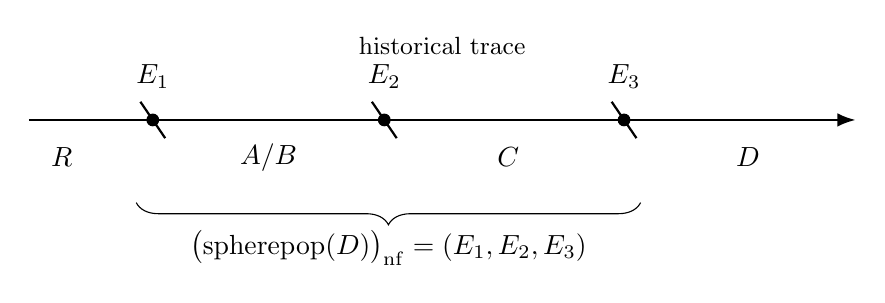
\begin{tikzpicture}[scale=1.05,>=Latex]
  \draw[thick,->] (0,0) -- (10,0);
  \filldraw (1.5,0) circle (2pt) node[above=8pt] {$E_1$};
  \filldraw (4.3,0) circle (2pt) node[above=8pt] {$E_2$};
  \filldraw (7.2,0) circle (2pt) node[above=8pt] {$E_3$};
  \node at (0.4,-0.45) {$R$};
  \node at (2.9,-0.45) {$A/B$};
  \node at (5.8,-0.45) {$C$};
  \node at (8.7,-0.45) {$D$};
  \foreach \x in {1.5,4.3,7.2} {
    \draw[thick] (\x-0.15,0.22) -- (\x+0.15,-0.22);
  }
  \draw[decorate,decoration={brace,mirror,amplitude=8pt}]
    (1.3,-1.0) -- (7.4,-1.0);
  \node at (4.35,-1.55)
    {$\bigl(\mathrm{spherepop}(D)\bigr)_{\mathrm{nf}}=(E_1,E_2,E_3)$};
  \node at (5,0.9) {\small historical trace};
\end{tikzpicture}
\caption{A geometric representation of an event word as an irreversible trace.
Tick marks indicate irreversible transitions; the brace records the
corresponding normal form.}
\label{fig:trace}
\end{figure}

The geometric picture reinforces a fundamental intuition: an object's position
on this trace cannot be recovered by inspecting the object alone.  Just as a
physical process that has dissipated energy cannot be run backwards to recover
the initial configuration, a Spherepop object does not carry within itself the
information necessary to reconstruct its generating history.  The normal form
is an external record, not an intrinsic property.

This historical criterion avoids several classical difficulties of set-based
ontology.  Objects in Spherepop are not defined by membership in collections
but by the irreversible sequences that produced them.  The ontology is
therefore inherently process-based: objects are histories rather than
containers, and the content of an object is its temporal structure rather than
its spatial extension.



\section{Possibility as the Preimage of History}
\label{sec:possibility-preimage}

The event-word formalism of Section~\ref{sec:eventwords} provides a complete
and canonical representation of object identity in terms of irreversible
sequences of transformations.  Each object $X$ is identified with a normal form
\[
  (\mathrm{spherepop}(X)) = (E_{i_1}, E_{i_2}, \dots, E_{i_k}),
\]
and identity is adjudicated by equality of these sequences.  This construction
is sufficient for distinguishing objects once their histories are given.  But it
leaves a prior question unanswered: what is the structure from which such
histories arise?  To ask what an event word records is already to presuppose
that it records something rather than being primitive.  This section makes the
answer precise.

The central claim is that an event history should be understood not as a
primitive object but as the irreversible boundary trace of a deeper process,
namely the progressive elimination of possibilities.  The event word is not
merely a record of what happened; it is the ordered residue of what has been
made impossible.  Identity as event history is therefore a derived notion: it
is what remains when possibility has been progressively collapsed.

\subsection{The State Pair}

At any stage of a process we do not have merely a partial history, but a pair
consisting of what has already been irrevocably committed and what still remains
open.  This motivates the following definition.

\begin{definition}[Spherepop state]
\label{def:statepair}
A \emph{Spherepop state} at stage $t$ is a pair
\[
  (\Omega_t, H_t),
\]
where $\Omega_t$ is a finite set of admissible events representing the residual
option space, and $H_t \in \mathcal{E}^{*}$ is the event word representing the
committed history accumulated up to stage $t$.
\end{definition}

The two components play fundamentally different structural roles.  The history
$H_t$ is an ordered, append-only record of irreversible commitments; it carries
the full ordering structure established in Section~\ref{sec:eventwords} and
required by the DAG construction to follow in Section~\ref{sec:dags}.  The
option space $\Omega_t$ is an unordered set, because the future has not yet
been differentiated by the act of choice: the possibilities that remain do not
yet stand in any causal relation to each other, and imposing an order on them
would be to read the future backwards from the past.

This asymmetry between the ordered history and the unordered option space is
not a notational convention; it is the formal expression of the asymmetry of
time.  The past has a definite sequence because it is constituted by the
specific order in which exclusions occurred.  The future is an unordered cloud
because no commitment has yet been made that would differentiate one remaining
possibility from another.

\subsection{The Axioms of Irreversible Evolution}

Three axioms govern the evolution of the state pair.  They are not independent
stipulations but consequences of taking irreversibility seriously as the
foundational property of Spherepop processes.

\begin{axiom}[Irreversibility]
\label{ax:irrev}
For any admissible transition from stage $t$ to stage $t+1$, the option
space satisfies $\Omega_{t+1} \subseteq \Omega_t$ and the commitment history
satisfies $H_{t+1} = H_t \cdot w$ for some non-empty extension
$w \in \mathcal{E}^{*}$.  No operation within the formalism can enlarge
$\Omega_t$ or remove any element from $H_t$.
\end{axiom}

\begin{axiom}[Exclusion Primitivity]
\label{ax:exclusion}
The only admissible operation on $\Omega_t$ is the removal of elements.
An event that has been excluded from the option space does not return.
Exclusion is primitive; there is no complementary inclusion operation.
\end{axiom}

\begin{axiom}[History Sufficiency]
\label{ax:sufficiency}
Every observable property of the process at stage $t$ factors through the
commitment history $H_t$ together with a fixed initial state $s_0$.  No
observable property depends on $\Omega_t$ independently of the history that
produced the current option space by successive exclusion from $\Omega_0$.
\end{axiom}

Axiom~\ref{ax:irrev} encodes the directed acyclic structure that will be
made precise in Section~\ref{sec:dags}: because the option space can only
shrink and the history can only grow, the evolution of the state pair traces
a path through a strictly ordered sequence of states, with no cycles and no
backward steps.  Axiom~\ref{ax:exclusion} ensures that the boundary of the
excluded region grows monotonically; combined with Axiom~\ref{ax:irrev}, it
implies that every event word is a record of irreversible decisions.
Axiom~\ref{ax:sufficiency} ensures that the pair $(\Omega_t, H_t)$ is not
merely a bookkeeping device but carries the full semantic content of the
process: state is reconstructible from history, and the option space is
reconstructible from the history together with knowledge of what was initially
available.

\subsection{Event Words as Boundary Traces}

With the state pair in hand, we can now give a precise account of what the
Spherepop normal form records.

\begin{proposition}[History as projection of possibility dynamics]
\label{prop:history-projection}
Let $(\Omega_0, \varepsilon)$ be an initial state and let
\[
  (\Omega_0, \varepsilon) \;\longrightarrow\;
  (\Omega_1, H_1) \;\longrightarrow\; \cdots \;\longrightarrow\;
  (\Omega_k, H_k)
\]
be a sequence of irreversible transitions satisfying Axiom~\ref{ax:irrev}.
Then the event word $H_k = (E_{i_1}, \ldots, E_{i_k})$ is the ordered record
of the successive contractions
\[
  \Omega_0 \supseteq \Omega_1 \supseteq \cdots \supseteq \Omega_k,
\]
and the normal form $(\mathrm{spherepop}(X))_{\mathrm{nf}} = H_k$ encodes
the trajectory of the option space under monotone exclusion.
\end{proposition}

\begin{proof}
Each transition appends exactly one event to the history and removes at least
that event from the option space by Axiom~\ref{ax:irrev} and
Axiom~\ref{ax:exclusion}.  The sequence of appended events is precisely
$(E_{i_1}, \ldots, E_{i_k})$ and the sequence of option spaces is
$\Omega_0 \supseteq \cdots \supseteq \Omega_k$.  The event word is therefore
a complete record of the exclusion sequence.
\end{proof}

The normal form $(\mathrm{spherepop}(X))$ is in this sense a boundary object:
it records the sequence of exclusions but not the internal structure of the
option space at each stage.  Two distinct trajectories of $\Omega_t$ may
produce identical event words if they eliminate the same events in the same
order, but the event word itself contains no explicit representation of the
alternatives that were available but not taken.  This is precisely the
information that is lost in the projection from full dynamics to boundary
trace, and it is the formal content of the historical reconstruction problem
taken up in Section~\ref{sec:reconstruction}.

\subsection{Identity as Projection}

The reformulation of history as a projection from possibility dynamics allows
us to factor the construction of identity into two stages.  The first stage is
dynamical: a process evolves within the space of possibility-history pairs,
generating a trajectory through states of diminishing possibility and growing
commitment.  The second stage is projective: the identity of the resulting
object is obtained by discarding the option space and retaining only the
accumulated commitment history.

\begin{definition}[History projection]
\label{def:hist-proj}
The \emph{history projection} is the map
\[
  \Pi_{\mathrm{hist}} : (\Omega_t, H_t) \;\longmapsto\; H_t
\]
which discards all information about the residual option space and retains
only the ordered commitment history.
\end{definition}

The Spherepop identity criterion is then a statement about the image of this
projection: two objects are identical precisely when their histories coincide
under $\Pi_{\mathrm{hist}}$, that is, when the ordered record of their
successive exclusions is the same.  Different trajectories through the space
of possibility-history pairs that happen to produce the same sequence of
exclusions yield the same Spherepop identity, because $\Pi_{\mathrm{hist}}$
maps them to the same image.  This is not an approximation or a convention;
it is the formal sense in which history is what matters and residual
possibility is not part of the identity of a completed object.

\subsection{Consequence: Irreversibility as Definitional}

The key insight that this reformulation yields is that irreversibility is not
an external constraint imposed on the formalism but a definitional feature of
the projection $\Pi_{\mathrm{hist}}$.  An event word grows by appending; it
does not shrink.  An option space shrinks by exclusion; it does not grow.
The asymmetry between them is built into the definition of the state pair and
the axioms that govern it.  When we say that Spherepop objects have irreversible
histories, we are saying that history is the image of a fundamentally directional
process, one that moves from larger to smaller option spaces and from shorter
to longer commitment records, and that the arrow of this process is not
reversible because there is no operation in the formalism that takes a smaller
option space back to a larger one or a longer history back to a shorter one.

The event-word formalism of Section~\ref{sec:eventwords}, the DAG structure of
Section~\ref{sec:dags}, and the normalization theory of
Section~\ref{sec:normalization} all describe properties of the image of
$\Pi_{\mathrm{hist}}$.  What the present section establishes is the preimage:
the space of possibility-history dynamics from which those images are derived.
Every subsequent formal development in this essay can be read in two registers
simultaneously---as a statement about event words, which is the register of the
boundary trace, and as a statement about the trajectories in $(\Omega_t, H_t)$
space that produced those event words.

\section{Entropy as Contraction of Possibility}
\label{sec:entropy}

The previous section reinterpreted event histories as boundary traces of a
deeper dynamical process: the progressive contraction of a space of
possibilities.  We now derive the entropy measure of a history directly from
this contraction.  Rather than introducing entropy as an external quantity
assigned to events by a weight function, we show that it emerges naturally
from the geometry of option spaces under successive exclusion.

\subsection{Entropy as Logarithmic Volume of Possibility}

Let $(\Omega_0, \varepsilon)$ be an initial state and let $\Omega_t$ denote
the residual option space at stage $t$.  We define the possibility-entropy
at stage $t$ by
\[
  S_t \;=\; \log |\Omega_t|,
\]
where $|\Omega_t|$ is the cardinality of the remaining possibilities.  If
$\Omega_t$ carries a probability measure $\mu$ reflecting the relative
accessibility of remaining events, the definition extends to
$S_t = \log \mu(\Omega_t)$, but for most purposes the cardinality version
suffices.

This definition captures the intuitive idea that entropy measures the size of
the future.  A large option space corresponds to high possibility-entropy: many
distinct continuations remain open.  A small option space corresponds to low
possibility-entropy: the future has become highly constrained by the
commitments already made.

\subsection{Irreversibility as Entropy Descent}

Under Axiom~\ref{ax:irrev}, the option space shrinks monotonically:
$\Omega_{t+1} \subseteq \Omega_t$.  It follows immediately that
\[
  S_{t+1} \;=\; \log |\Omega_{t+1}| \;\leq\; \log |\Omega_t| \;=\; S_t.
\]
Possibility-entropy is non-increasing along every admissible trajectory.
This is not a contingent fact about particular systems but a direct consequence
of the axioms.

This relationship to classical entropy deserves comment.  In thermodynamics,
entropy increases along irreversible processes: information about the detailed
microstate is dispersed into inaccessible degrees of freedom.  Here, entropy
decreases along irreversible processes: accessible alternatives are progressively
eliminated.  The two are dual descriptions of the same underlying directionality.
What is lost from the option space is exactly what is dispersed into the
irrecoverable past.  The event word records the eliminations; the entropy
measures their cumulative magnitude.

\subsection{Event Contributions as Entropy Drops}

Each transition contributes a discrete reduction in possibility-entropy.  For
a transition $(\Omega_t, H_t) \to (\Omega_{t+1}, H_{t+1})$, the entropy
drop is
\[
  \Delta S_t \;=\; S_{t+1} - S_t
  \;=\; \log \frac{|\Omega_{t+1}|}{|\Omega_t|} \;\leq\; 0.
\]

We associate to each event $E_{i_j}$ appended at step $j$ a natural weight
derived from the option space dynamics:
\[
  w(E_{i_j}) \;=\; -\Delta S_{j-1}
  \;=\; \log \frac{|\Omega_{j-1}|}{|\Omega_j|}.
\]

This weight measures how many possibilities are eliminated when the event
occurs.  An event that reduces a large option space by a single element carries
small weight; an event that halves the option space carries weight $\log 2$.

Summing over a complete history $H_k = (E_{i_1}, \dots, E_{i_k})$:
\[
  \sum_{j=1}^{k} w(E_{i_j})
  \;=\; \sum_{j=1}^{k} \log \frac{|\Omega_{j-1}|}{|\Omega_j|}
  \;=\; \log \frac{|\Omega_0|}{|\Omega_k|}.
\]

The total historical weight is exactly the log-ratio of the initial to the
terminal option space: the total contraction of possibility that the history
represents.  The event word does not merely record what happened; it encodes
the cumulative loss of possibility required to produce the object.

\subsection{Historical Complexity Derived from Contraction}

The definition of historical complexity can now be given a precise geometric
form.  For an object $X$ arising from a trajectory with initial state
$\Omega_0$ and terminal option space $\Omega_k$, define
\[
  S(X) \;=\; \log \frac{|\Omega_0|}{|\Omega_k|}.
\]

This is the logarithm of the ratio by which the space of possibilities has
been contracted in order to produce $X$.  Objects with high $S(X)$ arose
from trajectories that carved deeply into the option space, leaving behind a
narrow corridor of remaining alternatives.  Objects with low $S(X)$ arose
from histories that barely constrained the future.

This definition subsumes the earlier formulation of complexity as a weighted
event count.  The event-count formulation, which assigned an external weight
$w : \mathcal{E} \to \mathbb{R}_{\geq 0}$ to each event type and summed these
weights over the history, is recovered as a special case by choosing $w(E)$ to
approximate the entropy drop $-\Delta S$ associated with each event type.  The
present formulation is more fundamental because it derives the weights from the
option space dynamics rather than assigning them externally.

\subsection{Geometric Interpretation: Widening Trace as Illusion}

The earlier geometric picture of historical complexity as a widening trace
(described further in Section~\ref{sec:landscape}) can now be understood more
precisely.  The apparent widening of the trace as events accumulate reflects
the growing informational content of the commitment history: each additional
event adds information to the record of what has been excluded.  But from the
perspective of the option space, the picture is exactly reversed: the option
space narrows as the history widens.

The widening trace and the narrowing option space are dual representations of
the same process, viewed from opposite ends of the projection $\Pi_{\mathrm{hist}}$
introduced in Section~\ref{sec:possibility-preimage}.  The widening trace is
the image under that projection; the narrowing option space is the domain.  The
apparent visual metaphor of growth is therefore a representation of the history
side of the dynamics; the underlying reality of the possibility side is one of
contraction.

\subsection{Toward Responsibility Weights}

The entropy formulation treats all eliminations as quantitatively comparable,
differing only in magnitude.  But events differ not only in how much possibility
they eliminate, but in the character of that elimination: whether it arises from
structural constraint, from deliberate commitment, or from principled refusal.
This distinction cannot be captured by the entropy weight $w(E)$ alone, because
that weight is defined entirely by the cardinality change in $\Omega_t$ and is
indifferent to the provenance of the exclusion.

To capture this distinction, we introduce a refinement of the weight structure.
Each event $E$ in a history carries not only an entropy weight $w(E)$ derived
from the contraction of the option space, but a responsibility weight $\rho(E)$
that records the degree to which the elimination of possibilities is attributable
to the system's own agency.  The total responsibility of an object is then
\[
  \mathcal{R}(X) \;=\; \sum_{j=1}^{k} \rho(E_{i_j}),
\]
which provides a second independent measure on histories running in parallel
with the entropy measure $S(X)$.  While $S(X)$ measures how much possibility
has been contracted, $\mathcal{R}(X)$ measures who or what is answerable for
that contraction.

Both measures arise from the same underlying structure---the irreversible
contraction of $\Omega_t$---but they answer different questions about that
structure.  One asks about magnitude; the other asks about provenance.  The
full elaboration of the responsibility measure, including the operator
vocabulary that distinguishes the types of exclusion from which it arises, is
developed in Section~\ref{sec:opvocab}.
\section{A Categorical Interpretation of Spherepop Histories}
\label{sec:categorical}

The representation of objects as event words suggests an immediate connection
with category theory, where the primacy of morphisms over objects is a
foundational methodological principle \citep{MacLane1998}.  In the categorical
framework, processes rather than states are primary; objects emerge as the
sources and targets of transformations, and the composition of morphisms
encodes the sequential structure of processes.  This perspective aligns
precisely with the Spherepop principle that identity is grounded in generative
history.

Let $\mathcal{C}$ be a category whose objects represent regions or
configurations of a system and whose morphisms represent irreversible events.
An event
\[
  E : X \rightarrow Y
\]
corresponds to a transformation that produces the region $Y$ from the region
$X$.  If two events occur sequentially,
\[
  E_1 : X \rightarrow Y, \qquad E_2 : Y \rightarrow Z,
\]
their categorical composition
\[
  E_2 \circ E_1 : X \rightarrow Z
\]
represents the combined historical process producing $Z$ from $X$.  In this
formulation, the event word introduced in Section~\ref{sec:eventwords}
corresponds precisely to a composition of morphisms, and the normal form of
an object is the morphism that takes the initial state to the present one.

Branching and merging events, which are prominent features of the worked
example, correspond to familiar categorical constructions.  A split event
\[
  E_1 : R \rightarrow A \sqcup B
\]
resembles a coproduct-like branching in which a single region gives rise to
multiple descendants, while a merge event
\[
  E_3 : (B, C) \rightarrow D
\]
resembles a pushout-like construction in which two regions produced from a
common ancestor are combined into a new one \citep{MacLane1998, Spivak2014}.
The precise categorical status of these constructions is examined further in
Section~\ref{sec:pushouts}; for present purposes it suffices to note that
the full history of the worked example forms a diagram in $\mathcal{C}$ of
the shape illustrated in Figure~\ref{fig:categorical}.

\begin{figure}[ht]
\centering
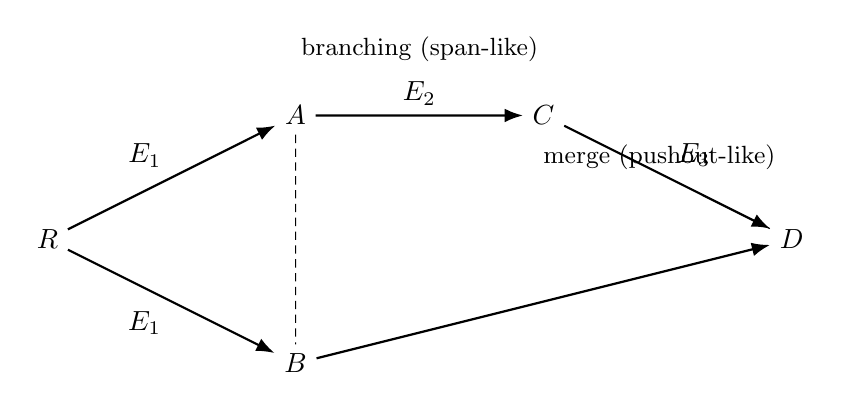
\begin{tikzpicture}[scale=1.05,>=Latex]
  \node (R) at (0,0)   {$R$};
  \node (A) at (3,1.5) {$A$};
  \node (B) at (3,-1.5){$B$};
  \node (C) at (6,1.5) {$C$};
  \node (D) at (9,0)   {$D$};
  \draw[thick,->] (R) -- node[above left]  {$E_1$} (A);
  \draw[thick,->] (R) -- node[below left]  {$E_1$} (B);
  \draw[thick,->] (A) -- node[above]       {$E_2$} (C);
  \draw[thick,->] (B) -- (D);
  \draw[thick,->] (C) -- node[above right] {$E_3$} (D);
  \draw[densely dashed] (A) -- (B);
  \draw[densely dashed] (C) -- (D);
  \node at (4.5,2.3)  {\small branching (span-like)};
  \node at (7.4,1.0)  {\small merge (pushout-like)};
\end{tikzpicture}
\caption{A categorical diagram of the worked example.  The split event $E_1$
produces a span, while the merge event $E_3$ completes a pushout-like
construction.  The identity of $D$ is determined by the entire diagram, not
merely by the node $D$ in isolation.}
\label{fig:categorical}
\end{figure}

From this perspective, the identity of an object is determined by the entire
diagram of morphisms that generated it.  Two objects are identical precisely
when the diagrams representing their histories are identical, up to equality of
morphisms.  This is a stronger condition than structural isomorphism of the
resulting objects; it requires agreement at every stage of the generative
process.

The categorical viewpoint also clarifies why Spherepop naturally produces
directed acyclic event graphs.  Cycles in a morphism-composition diagram would
correspond to reversible processes, since a path
\[
  X \rightarrow Y \rightarrow \dots \rightarrow X
\]
implies the existence of a composite morphism returning from $X$ to itself.  In
a setting where morphisms represent irreversible transformations, such a cycle
would violate the irreversibility condition.  The absence of cycles is therefore
not merely a convenient property but a structural consequence of the physical
or computational assumption that the events under consideration are
irreversible.  The relationship between irreversibility and directed acyclicity
is developed further in Section~\ref{sec:dags}, and the connection to entropy
is examined in Section~\ref{sec:entropy}.

\citet{BaezStay2010} describe in detail the deep correspondences among physics,
topology, logic, and computation through the ``Rosetta Stone'' of categorical
structures; the Spherepop framework sits naturally within the physical and
computational columns of that correspondence, where morphisms encode processes
and composition encodes sequential execution.


\section{Event Graphs and Directed Acyclic Structure}
\label{sec:dags}

Linear event words provide a correct representation of histories in which each
event has at most one predecessor and at most one successor.  The processes
encountered in practice, however, frequently involve branching and merging: a
single region may give rise to multiple descendants, and multiple regions may
combine to produce a single new one.  In such cases the linear notation,
though applicable after a suitable ordering is imposed, obscures the parallel
structure of the history.  The natural representation is a directed graph.

\begin{definition}[Event graph]
An \emph{event graph} is a directed graph $G = (V, \mathcal{E})$ in which the
vertices $V$ represent regions and each directed edge $X \rightarrow Y$
represents an irreversible event producing the region $Y$ from the region $X$.
\end{definition}

When events produce multiple descendants or require multiple inputs, the
corresponding vertices in $G$ carry multiple outgoing or incoming edges
respectively.  The complete generative history of a system is encoded in the
global structure of $G$ rather than in any single path through it.

\begin{proposition}[Directed acyclicity]
Every Spherepop event graph is a directed acyclic graph (DAG).
\end{proposition}

\begin{proof}
Suppose for contradiction that $G$ contains a directed cycle
$X \rightarrow Y \rightarrow \cdots \rightarrow X$.  Then there exists a
composite event morphism that maps $X$ to itself, implying that the
transformation can be applied repeatedly to yield a reversible process
taking $X$ back to a state indistinguishable from $X$.  Since every
Spherepop event is irreversible by definition, such a composite cannot exist.
Consequently no directed cycle can occur in $G$.
\end{proof}

The directed acyclic property is not merely a convenience; it is the formal
analogue of the thermodynamic irreversibility condition formalized in
Section~\ref{sec:entropy}.  Every finite DAG admits a topological ordering, and
it is precisely this ordering that will be exploited by the normalization
procedure of Section~\ref{sec:normalization} to produce canonical event words
from branching histories.

Given an object $X$ appearing as a vertex in $G$, its identity is determined
not by the local properties of the vertex but by the global structure of the
subgraph that generated it.  Formally, let $\mathrm{Anc}(X)$ denote the set of
all vertices from which $X$ is reachable by a directed path in $G$.  The
\emph{ancestral subgraph} of $X$ is the induced subgraph
\[
  G_X = G[\mathrm{Anc}(X) \cup \{X\}]
\]
containing all vertices that contributed, directly or indirectly, to the
production of $X$.

\begin{definition}[Spherepop identity, graphical formulation]
Two objects $X$ and $Y$ are Spherepop-identical if and only if their
ancestral subgraphs $G_X$ and $G_Y$ are isomorphic as directed graphs with
edges labelled by event types.
\end{definition}

This definition subsumes the event-word formulation of Section~\ref{sec:eventwords}
as a special case: when histories are linear (no branching or merging), the
ancestral subgraph reduces to a directed path, and graph isomorphism reduces to
equality of the corresponding event sequences.

Figure~\ref{fig:dag} illustrates a more complex event graph containing multiple
levels of branching.  The terminal object $Z$ is determined by the entire
layered DAG structure feeding into it.  Different subsets of the graph
characterise different terminal objects; the identity criterion requires that
the complete ancestral subgraph, not merely the immediately preceding events,
be taken into account.

\begin{figure}[ht]
\centering
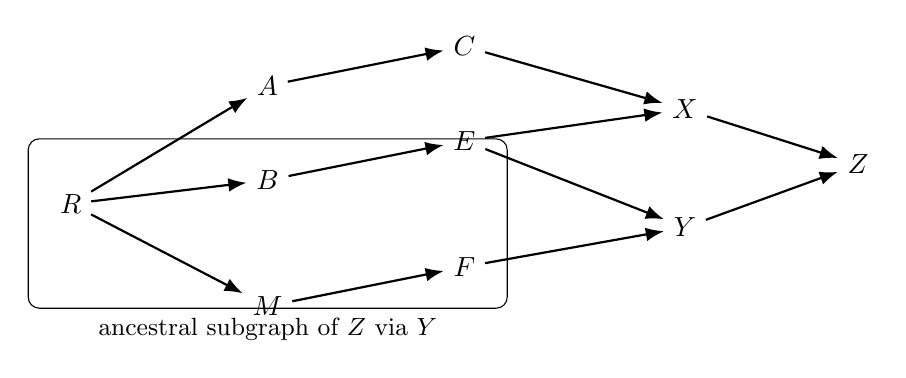
\begin{tikzpicture}[scale=1.0,>=Latex]
  \node (R) at (0,0)    {$R$};
  \node (A) at (2.5,1.5){$A$};
  \node (B) at (2.5,0.3){$B$};
  \node (M) at (2.5,-1.3){$M$};
  \node (C) at (5,2.0)  {$C$};
  \node (E) at (5,0.8)  {$E$};
  \node (F) at (5,-0.8) {$F$};
  \node (X) at (7.8,1.2){$X$};
  \node (Y) at (7.8,-0.3){$Y$};
  \node (Z) at (10,0.5) {$Z$};
  \foreach \u/\v in {R/A,R/B,R/M,A/C,B/E,M/F,C/X,E/X,E/Y,F/Y,X/Z,Y/Z}
    \draw[thick,->] (\u) -- (\v);
  \begin{scope}[on background layer]
    \node[draw,rounded corners,inner sep=8pt,
          fit=(R)(B)(F),
          label=below:{\small ancestral subgraph of $Z$ via $Y$}] {};
  \end{scope}
\end{tikzpicture}
\caption{A layered directed acyclic event graph.  The identity of the terminal
object $Z$ is determined by the entire ancestral subgraph that feeds into it,
not merely by its immediate predecessors $X$ and $Y$.}
\label{fig:dag}
\end{figure}

The DAG representation also clarifies the relationship between the event-word
notation and the diagrammatic structure.  A linear event word corresponds to a
directed path through the DAG.  Branching corresponds to a vertex with multiple
outgoing edges, and merging corresponds to a vertex with multiple incoming
edges.  The graph therefore provides a complete representation of the causal
structure, while the event word provides a linear serialization of that
structure.  The correspondence between these two representations is the subject
of the normalization theory in Section~\ref{sec:normalization}, where it is
shown that every event graph admits a canonical linear serialization.


\section{Normalization and Canonical Representation}
\label{sec:normalization}

The event graph representation captures the full causal structure of a history,
but different textual descriptions of the same graph may arise depending on
the order in which causally independent events are recorded.  If two events
act on disjoint regions without either depending on the output of the other,
then listing them in either order produces an equivalent description of the
same causal structure.  This equivalence must be recognized formally if the
identity criterion is to be stable under changes of representation.

\begin{definition}[Event independence]
Two events $E_i, E_j \in \mathcal{E}$ are \emph{independent}, written
$E_i \parallel E_j$, if neither event requires the output of the other as
input; equivalently, there is no directed path between $E_i$ and $E_j$ in the
event graph.
\end{definition}

Independent events may appear in either order in a linear serialization of the
event graph without altering the graph's structure.  This motivates the
following rewriting rule, which will be made precise in Appendix~\ref{app:rewriting}:

\[
  (E_i, E_j) \;\longrightarrow\; (E_j, E_i)
  \quad \text{whenever } E_i \parallel E_j.
\]

Two event words are \emph{causally equivalent} if they are related by a finite
sequence of such commutation steps.  The normalization procedure selects a
canonical representative from each causal equivalence class.

\begin{definition}[Spherepop normal form, canonical]
The \emph{Spherepop normal form} of an object $X$ is the event word
\[
  (\text{spherepop}(X))_{\mathrm{nf}}
\]
obtained by computing a topological ordering of the event graph $G_X$ and
serializing the events in that order, breaking ties consistently according to
a fixed deterministic convention on event labels.
\end{definition}

Because every finite DAG admits a topological ordering, and because the
normalization procedure is deterministic, the normal form is well-defined for
every Spherepop object.  The canonical identity condition becomes:
\[
  X \equiv Y
  \quad\Longleftrightarrow\quad
  (\text{spherepop}(X))_{\mathrm{nf}} = (\text{spherepop}(Y))_{\mathrm{nf}}.
\]

Two objects are identical exactly when their normalized event histories
coincide, regardless of the particular serialization that may have been used
to describe their histories in the first instance.

Figure~\ref{fig:normalization} illustrates this point concretely.  Two
syntactically different presentations of the same history---one listing $E_i$
before $E_j$ and the other listing $E_j$ before $E_i$ on two parallel
branches---both normalize to the same canonical form, because the two events
are independent and the topological ordering convention resolves the tie
deterministically.

\begin{figure}[ht]
\centering
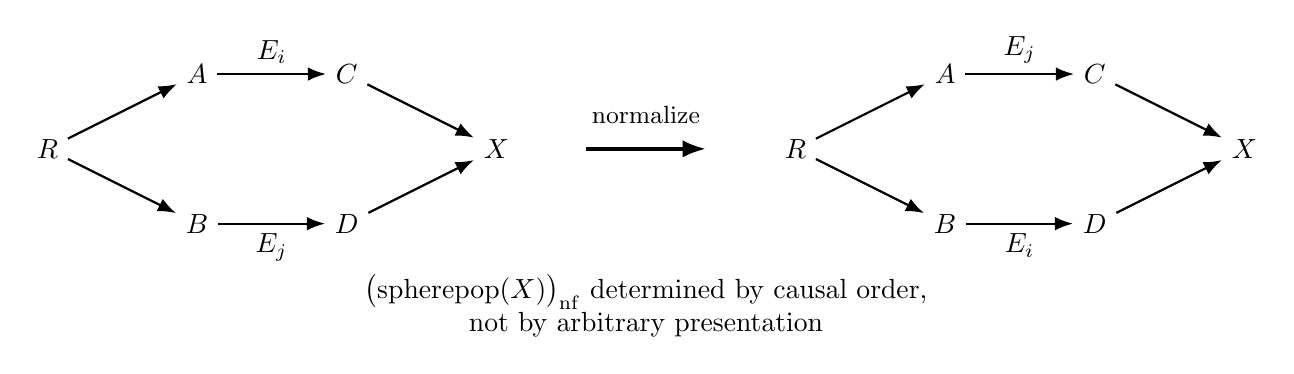
\begin{tikzpicture}[scale=0.95,>=Latex]
  \node (R1) at (0,0)   {$R$};
  \node (A1) at (2,1)   {$A$};
  \node (B1) at (2,-1)  {$B$};
  \node (C1) at (4,1)   {$C$};
  \node (D1) at (4,-1)  {$D$};
  \node (X1) at (6,0)   {$X$};
  \draw[thick,->] (R1)--(A1);
  \draw[thick,->] (R1)--(B1);
  \draw[thick,->] (A1)-- node[above] {$E_i$} (C1);
  \draw[thick,->] (B1)-- node[below] {$E_j$} (D1);
  \draw[thick,->] (C1)--(X1);
  \draw[thick,->] (D1)--(X1);
  \node (R2) at (10,0)  {$R$};
  \node (A2) at (12,1)  {$A$};
  \node (B2) at (12,-1) {$B$};
  \node (C2) at (14,1)  {$C$};
  \node (D2) at (14,-1) {$D$};
  \node (X2) at (16,0)  {$X$};
  \draw[thick,->] (R2)--(A2);
  \draw[thick,->] (R2)--(B2);
  \draw[thick,->] (A2)-- node[above] {$E_j$} (C2);
  \draw[thick,->] (B2)-- node[below] {$E_i$} (D2);
  \draw[thick,->] (C2)--(X2);
  \draw[thick,->] (D2)--(X2);
  \draw[very thick,->] (7.2,0) -- (8.8,0);
  \node at (8,0.45) {\small normalize};
  \node[align=center] at (8,-2.1)
    {$\bigl(\mathrm{spherepop}(X)\bigr)_{\mathrm{nf}}$
     determined by causal order,\\not by arbitrary presentation};
\end{tikzpicture}
\caption{Two syntactically different presentations of independent events $E_i$
and $E_j$ encoding the same causal structure.  Normalization collapses both to
a single canonical form, since $E_i \parallel E_j$ implies their order may be
resolved by any fixed topological convention.}
\label{fig:normalization}
\end{figure}

The normalization procedure plays a role in Spherepop analogous to that of
canonical forms in other mathematical frameworks: reduced words in group theory,
row echelon form in linear algebra, beta-normal forms in the lambda calculus.
Each of these devices converts a syntactically diverse family of equivalent
expressions into a unique representative that can be compared directly.  In
Spherepop, the canonical form ensures that identity depends only on causal
structure rather than on the order in which an external observer happened to
record causally independent events.


\section{Functorial Perspectives on Event Histories}
\label{sec:functors}

The event graph representation and the normalization theory of
Section~\ref{sec:normalization} can be cast in a fully categorical language by
treating the process of mapping abstract causal structures onto concrete systems
as a functor.  This perspective, which draws on the categorical foundations
developed in \citet{MacLane1998} and elaborated in \citet{Spivak2014} and
\citet{BaezStay2010}, provides the most general formulation of Spherepop
semantics.

\begin{definition}[Causal history category]
Let $\mathcal{H}$ be a small category whose objects represent intermediate
regions or states in a history and whose morphisms represent irreversible
events.  Because the events are temporally ordered and irreversible, if there
exists a morphism $X \rightarrow Y$ in $\mathcal{H}$ then there cannot exist
a morphism $Y \rightarrow X$.  Such a category is called a \emph{causal
history category}.
\end{definition}

In practice, $\mathcal{H}$ may be constructed directly from the event graph
$G$ by interpreting vertices as objects and directed edges as generating
morphisms, with composition given by directed paths.  The temporal ordering
that the DAG structure imposes on $G$ corresponds to the ``no-back-morphism''
condition in $\mathcal{H}$.

\begin{definition}[Spherepop realization functor]
Let $\mathcal{C}$ be a category of regions, configurations, or system states.
A \emph{Spherepop realization} of the history $\mathcal{H}$ in $\mathcal{C}$
is a functor
\[
  F : \mathcal{H} \rightarrow \mathcal{C}.
\]
\end{definition}

The functor $F$ assigns to each node in the abstract causal history a concrete
object in $\mathcal{C}$, and to each event morphism the corresponding
transformation in the physical or computational system.  Functoriality ensures
that sequential composition of events in $\mathcal{H}$ corresponds exactly to
sequential composition of transformations in $\mathcal{C}$:
\[
  F(E_2 \circ E_1) = F(E_2) \circ F(E_1).
\]
This coherence condition is the categorical expression of the physical
requirement that the combined effect of two sequential events is the
composition of their individual effects, without hidden intermediate states.

Terminal objects of $\mathcal{H}$ correspond to the currently existing objects
of the system---those that have not been further transformed.  If $X$ is such a
terminal node, then $F(X)$ represents the concrete present state produced by
the entire chain of events that preceded it.  The identity of $F(X)$ as a
Spherepop object is determined jointly by $F$ and by the position of $X$ in
the causal diagram.

Figure~\ref{fig:functor} illustrates the functorial picture.  The abstract
causal history category $\mathcal{H}$ on the left carries the relational
structure of the history---which events preceded which---without specifying
their concrete content.  The functor $F$ maps this abstract structure into the
category $\mathcal{C}$ of realized regions on the right, where each abstract
node becomes a concrete object and each abstract morphism becomes a concrete
transformation.

\begin{figure}[ht]
\centering
\begin{tikzpicture}[scale=1.0,>=Latex]
  \node (hR) at (0,0)    {$r$};
  \node (hA) at (2,1.2)  {$a$};
  \node (hB) at (2,-1.2) {$b$};
  \node (hD) at (4,0)    {$d$};
  \draw[thick,->] (hR) -- (hA);
  \draw[thick,->] (hR) -- (hB);
  \draw[thick,->] (hA) -- (hD);
  \draw[thick,->] (hB) -- (hD);
  \node at (2,-2.0) {$\mathcal{H}$};
  \draw[very thick,->] (5.2,0) -- (8.3,0);
  \node at (6.7,0.45) {$F$};
  \node (cR) at (10,0)   [circle,draw,inner sep=1.5pt] {};
  \node (cA) at (12,1.4) [circle,draw,inner sep=1.5pt] {};
  \node (cB) at (12,-1.4)[circle,draw,inner sep=1.5pt] {};
  \node (cD) at (14,0)   [circle,draw,inner sep=1.5pt] {};
  \draw[thick,->] (cR) -- (cA);
  \draw[thick,->] (cR) -- (cB);
  \draw[thick,->] (cA) -- (cD);
  \draw[thick,->] (cB) -- (cD);
  \draw[densely dashed] (9.5,-0.5) ellipse (0.8 and 0.5);
  \draw[densely dashed] (12,1.4)   ellipse (0.9 and 0.55);
  \draw[densely dashed] (12,-1.4)  ellipse (0.9 and 0.55);
  \draw[densely dashed] (14,0)     ellipse (1.1 and 0.75);
  \node at (12,-2.0) {$\mathcal{C}$};
\end{tikzpicture}
\caption{A Spherepop history as a functor $F : \mathcal{H} \rightarrow \mathcal{C}$
from an abstract causal index category $\mathcal{H}$ to a category $\mathcal{C}$
of realized regions.  The abstract structure on the left encodes causal
precedence; the functor translates this into concrete transformations on the right.}
\label{fig:functor}
\end{figure}

The functorial formulation also provides a clean account of when two objects
should be considered identical.  Suppose
\[
  F_1 : \mathcal{H}_1 \rightarrow \mathcal{C}
  \quad\text{and}\quad
  F_2 : \mathcal{H}_2 \rightarrow \mathcal{C}
\]
are two realizations.  The resulting terminal objects coincide as Spherepop
objects when the normalized causal structures $\mathcal{H}_1$ and $\mathcal{H}_2$
are isomorphic as causal categories and the functors agree on the corresponding
morphisms under this isomorphism.  This condition recovers the normal-form
identity criterion of Section~\ref{sec:normalization} in categorical language:
it requires agreement not merely on terminal values but on the entire
structure of the generating process.

The functorial perspective also suggests how Spherepop should handle
abstraction.  Natural transformations between realizations---that is, morphisms
in the functor category $[\mathcal{H}, \mathcal{C}]$---correspond to
systematic reinterpretations of a history that change the concrete objects
assigned to nodes while preserving the relational structure.  In this way the
framework supports a hierarchy of increasingly abstract descriptions of the
same underlying causal history.


\section{Merge Events as Pushouts}
\label{sec:pushouts}

The merge events that appear prominently in Spherepop histories admit a precise
categorical characterization as pushout constructions.  A pushout in a category
$\mathcal{C}$ is the universal solution to the problem of combining two
morphisms that share a common source: given morphisms $f : R \rightarrow B$ and
$g : R \rightarrow C$, the pushout is an object $D$ together with morphisms
$B \rightarrow D$ and $C \rightarrow D$ such that the resulting square commutes
and $D$ is universal with this property \citep{MacLane1998}.

The connection to Spherepop is direct.  In the worked example of
Section~\ref{sec:worked}, the regions $B$ and $C$ both originated from the
common ancestor $R$ via the split event $E_1$.  The merge event $E_3$ then
combined $B$ and $C$ into the region $D$.  Categorically, this situation is
described by the commuting square
\[
\begin{tikzcd}
  R \arrow[r] \arrow[d] & C \arrow[d] \\
  B \arrow[r]           & D
\end{tikzcd}
\]
in which $D$ receives consistent morphisms from $B$ and $C$ and is universal
with this property.  The merge event $E_3$ corresponds precisely to the
completion of this pushout diagram.

\begin{figure}[ht]
\centering
\begin{tikzpicture}[scale=1.05,>=Latex]
  \node (R) at (0,0)  {$R$};
  \node (C) at (3,2)  {$C$};
  \node (B) at (3,-2) {$B$};
  \node (D) at (6,0)  {$D$};
  \draw[thick,->] (R) -- (C);
  \draw[thick,->] (R) -- (B);
  \draw[thick,->] (C) -- (D);
  \draw[thick,->] (B) -- (D);
  \node at (3,0) {$\square$};
\end{tikzpicture}
\caption{A merge event represented as a pushout-like square.  The common ancestor $R$
gives rise to $B$ and $C$ via the split event; the merge event $E_3$ completes
the square by producing the universal object $D$.}
\label{fig:pushout}
\end{figure}

The pushout interpretation makes precise the sense in which the identity of
$D$ depends on the entire commuting square rather than merely on the pair
$(B, C)$ considered in isolation.  Two regions $B'$ and $C'$ could be merged
to produce a region $D'$ with the same structural description as $D$, yet if
$B'$ and $C'$ arose from a different common ancestor $R'$, the resulting
pushout square would be different and $D'$ would be a different Spherepop
object.  The pushout construction thus encodes the relational history of the
merge event, not merely its output.

This observation connects to the broader theme of the paper.  In standard
set-theoretic or structural accounts of identity, two sets are equal when they
contain the same elements, regardless of how those elements were assembled.
The pushout characterization of merge events shows that in Spherepop the
corresponding condition is far stronger: the merged object must have arisen
from the same causal configuration, with the same common ancestor and the same
morphisms connecting it to its predecessors.

The pushout interpretation also interacts with the categorical coherence
conditions noted in Section~\ref{sec:functors}.  A realization functor
$F : \mathcal{H} \rightarrow \mathcal{C}$ that preserves pushouts maps each
merge event in the abstract history to a genuine pushout in the target
category.  When $\mathcal{C}$ is a category with all pushouts---for instance,
a category of sets or a category of topological spaces---this preservation
condition is automatically satisfied.  In physical applications, the relevant
category may not have all pushouts, and the question of when merge events can
be faithfully realized is a substantive one.


\section{Entropy Landscapes and Historical Trajectories}
\label{sec:landscape}

A complementary geometric interpretation of Spherepop histories arises from
the notion of an entropy landscape.  This interpretation is more impressionistic
than the category-theoretic treatment of preceding sections, but it connects
the formalism to physical intuitions about the role of irreversibility in
shaping the space of possible histories.

Let the configuration space of a system be represented as a manifold
$\mathcal{M}$ whose points correspond to possible structural states.  Define an
entropy-like functional
\[
  S : \mathcal{M} \rightarrow \mathbb{R}
\]
measuring the informational or thermodynamic complexity of each state.
Irreversible events may then be interpreted as transitions that move the system
along trajectories in $\mathcal{M}$ while generally increasing the value of
$S$.  The history of an object corresponds to a directed path through this
landscape, constrained to move in the direction of increasing $S$.

\begin{figure}[ht]
\centering
\begin{tikzpicture}[scale=1.0]
  \draw[thick] (-4,0) .. controls (-2,2) and (-1,1) .. (0,3)
               .. controls (1,5) and (3,3) .. (4,4);
  \draw[thick] (-4,0) .. controls (-2,-2) and (-1,-1) .. (0,-3)
               .. controls (1,-5) and (3,-3) .. (4,-4);
  \draw[very thick,->] (-3,0) -- (-1.5,0.8);
  \draw[very thick,->] (-1.5,0.8) -- (0.2,2.2);
  \draw[very thick,->] (0.2,2.2) -- (2.2,3.6);
  \node at (-3.2,0.4) {$E_1$};
  \node at (-1.5,1.4) {$E_2$};
  \node at (0.9,3.0)  {$E_3$};
  \node at (3.2,4.6)  {$S$};
\end{tikzpicture}
\caption{Event history interpreted as a directed trajectory across an entropy
landscape.  Each event corresponds to a transition along a path that generally
moves toward regions of higher entropy.  The topology of the landscape
constrains which transitions are possible.}
\label{fig:landscape}
\end{figure}

In this geometric picture, as illustrated in Figure~\ref{fig:landscape}, the
events $E_1$, $E_2$, $E_3$ correspond to successive steps along a trajectory
that climbs the entropy surface.  The shape of the landscape determines which
transitions are available at each point: a configuration at a local minimum of
$S$ that is not a global minimum may be accessible from some prior states but
inaccessible from others, and the question of reachability depends on the
full path taken up to that point.  This path-dependence is precisely the
feature that Spherepop captures through its event-word representation: the
normal form records not just the endpoint of the trajectory but the entire
path.

Critical points of the entropy functional may be interpreted as stable
structural configurations or attractor states.  The Spherepop history of an
object records the sequence of transitions that led to its current position on
the landscape, including which saddle points and ridges it passed through on
the way.  Two objects at the same configuration on the landscape but arriving
via different paths are therefore different Spherepop objects, even though a
purely spatial description would identify them.

The entropy landscape interpretation also suggests a connection to the theory
of gradient flows and Morse theory, where the topology of a functional landscape
constrains the structure of trajectories and the classification of critical
points.  Spherepop histories can in principle be studied using these geometric
tools to understand, for instance, which pairs of histories are deformable into
one another through the insertion or deletion of null events, or how the
topology of the causal DAG interacts with the geometry of the underlying
landscape.  This direction of generalization lies beyond the scope of the
present essay but suggests a rich programme of further investigation.


\section{Event Histories as Partial Orders}
\label{sec:posets}

The directed acyclic structure of Spherepop event graphs implies that each
history carries a natural partial order on its events.  Making this structure
explicit provides a useful bridge between the graph-theoretic and algebraic
representations of histories developed in previous sections, and connects the
Spherepop framework directly to classical order theory and the concurrency-
theoretic tradition of Mazurkiewicz \citep{Mazurkiewicz1987}.

Let $G = (V, \mathcal{E})$ be an event graph.  Define a binary relation
$\prec$ on the set of events by declaring
\[
  E_i \prec E_j
\]
whenever there exists a directed path from $E_i$ to $E_j$ in $G$.  The
following proposition is immediate from the DAG property established in
Section~\ref{sec:dags}.

\begin{proposition}
The relation $\prec$ is a strict partial order on the set of events of any
Spherepop history.
\end{proposition}

\begin{proof}
Irreflexivity holds because the event graph is acyclic: no event can appear
on a directed path that begins and ends at itself.  Asymmetry is immediate from
the same acyclicity: if $E_i \prec E_j$ then there is a directed path from
$E_i$ to $E_j$, and the existence of a directed path from $E_j$ to $E_i$ would
close a cycle.  Transitivity follows by concatenating directed paths: if
$E_i \prec E_j$ and $E_j \prec E_k$ then the composed path witnesses
$E_i \prec E_k$.
\end{proof}

Each Spherepop history therefore determines a partially ordered set
$(\mathcal{E}_X, \prec)$, called the \emph{causal poset} of $X$.  The
incomparable elements of this poset are precisely the mutually independent
events: two events $E_i$ and $E_j$ satisfy $E_i \parallel E_j$ if and only if
neither $E_i \prec E_j$ nor $E_j \prec E_i$.

The event words introduced in Section~\ref{sec:eventwords} can now be
interpreted with precision as \emph{linear extensions} of the causal poset.

\begin{definition}[Linear extension]
A \emph{linear extension} of $(\mathcal{E}_X, \prec)$ is a total ordering
$\leq$ of $\mathcal{E}_X$ such that $E_i \prec E_j$ implies $E_i \leq E_j$.
\end{definition}

Every topological ordering of the event graph $G_X$ corresponds to a linear
extension of the causal poset, and conversely every linear extension arises
from some topological ordering.  The collection of all linear extensions
therefore coincides precisely with the set of all event words that are causally
equivalent in the sense of Section~\ref{sec:normalization}: they represent
different serializations of the same partial order.

This observation reframes normalization in order-theoretic terms.  The
commutation rules that identify independent events are precisely the moves
that relate different linear extensions of the same poset.  The Spherepop
normal form selects a canonical linear extension by fixing a deterministic
rule for breaking incomparability ties.

The width of the causal poset, which counts the size of the largest antichain,
measures the maximal degree of parallelism in the history.  Dilworth's theorem
\citep{MacLane1998} states that the minimum number of chains needed to partition
the poset equals the width; in the Spherepop context this means that the most
compressed sequential description of a history requires at least as many
serialized chains as the width of its causal poset.  Wide histories represent
highly parallel processes that cannot be faithfully compressed into a single
short sequential trace.

The partial-order perspective thus provides the algebraic underpinning for both
the normalization theory and the complexity measures developed in the next
section, tying these constructions to the classical theory of posets and their
linear extensions.


\section{Historical Complexity Measures}
\label{sec:complexity}

The entropy measure $S(X)$ introduced in Section~\ref{sec:entropy} captures
the cumulative informational weight of a history by summing the contributions
of individual events.  A complementary family of measures can be derived
directly from the structure of the causal poset $(\mathcal{E}_X, \prec)$
introduced in Section~\ref{sec:posets}.  These graph-theoretic quantities
characterize the structural complexity of a history independently of any
specific thermodynamic or informational interpretation.

\begin{definition}[Historical depth]
The \emph{depth} of an object $X$ is the length of the longest directed path
in its ancestral event graph:
\[
  \mathrm{depth}(X) = \max\{\,|p| \mid p \text{ is a directed path in } G_X\,\}.
\]
\end{definition}

Depth measures the maximal sequential chain of irreversible events separating
$X$ from its ultimate ancestor.  In a purely linear history depth coincides
with the length of the event word, but in branching histories depth may be
significantly smaller than the total event count, since many events may proceed
in parallel.

\begin{definition}[Historical width]
The \emph{width} of the history of $X$ is the size of the largest antichain in
the causal poset:
\[
  \mathrm{width}(X) = \max\{\,|A| \mid A \subseteq \mathcal{E}(G_X)
  \text{ is an antichain}\,\}.
\]
\end{definition}

Width measures the maximal degree of concurrent activity present in the
history.  A history with large width contains many independent events that
could in principle occur simultaneously; a history with width one is entirely
sequential.

\begin{definition}[Branching factor]
The \emph{branching factor} of the history of $X$ is the maximum number of
outgoing edges from any vertex in $G_X$.
\end{definition}

Branching events correspond to moments at which the system diversifies into
multiple descendant configurations.  A high branching factor indicates that
individual transformations generate large numbers of descendants, producing
rapidly widening event trees.

These three quantities interact in informative ways.  By Dilworth's theorem,
as noted in Section~\ref{sec:posets}, the minimum number of chains required to
cover the causal poset equals the width; consequently $\mathrm{depth}(X)
\cdot \mathrm{width}(X)$ provides a lower bound on the total number of events
in the history.  Conversely, histories in which depth and width are both small
are in a precise sense efficiently compressed: they achieve their complexity
through neither excessive sequentiality nor excessive concurrency.

Beyond these three measures one may define finer invariants.  The
\emph{entropy growth rate} of a history is the ratio $S(X) / \mathrm{depth}(X)$,
measuring the average thermodynamic cost per sequential step.  The
\emph{causal density}, defined as the ratio of the number of edges to the
number of vertices in $G_X$, captures how heavily constrained the event graph
is by precedence relations.  Histories with high causal density are those in
which most events depend on most prior events; histories with low causal density
are those with sparse causal dependencies and therefore high parallelism.

Together, the complexity measures of this section provide a basic vocabulary
for comparing the structural profiles of different generative processes.  They
complement the entropy functional by describing not the thermodynamic cost of
a history but its combinatorial shape---whether it is deep or shallow, narrow
or wide, densely or sparsely connected.  A full complexity theory of Spherepop
histories would develop these measures systematically, establishing bounds on
their interactions and identifying which profiles are achievable under given
constraints on the event signature.


\section{Operational Semantics of Spherepop}
\label{sec:operational}

The preceding sections have treated Spherepop histories primarily as static
structures: event words, partial orders, directed graphs, and categorical
diagrams.  It is equally important to understand the framework dynamically, as
an operational system in which configurations evolve through discrete
transitions.  This section introduces a small-step operational semantics for
Spherepop that makes the execution model explicit and connects the historical
identity criterion to the standard vocabulary of process calculi and labeled
transition systems \citep{Abramsky1994}.

Let $\Sigma$ denote the set of possible system configurations.  A
\emph{labeled transition system} (LTS) for Spherepop consists of a set
$\Sigma$ of configurations, a set $\mathcal{E}$ of event labels, and a
transition relation
\[
  {\xrightarrow{E}} \;\subseteq\; \Sigma \times \mathcal{E} \times \Sigma,
\]
written $X \xrightarrow{E} Y$ when the event $E$ transforms configuration $X$
into configuration $Y$.  The irreversibility assumption requires that the
relation contain no pair of transitions $X \xrightarrow{E} Y$ and
$Y \xrightarrow{E'} X$ for any events $E$ and $E'$.

A Spherepop history arises as an execution trace of this LTS.  Starting from
an initial configuration $X_0$, a sequence of enabled transitions
\[
  X_0 \xrightarrow{E_1} X_1
      \xrightarrow{E_2} X_2
      \xrightarrow{E_3} \cdots
      \xrightarrow{E_k} X_k
\]
generates the object $X_k$.  The normal form of $X_k$ is the trace of event
labels produced by this execution:
\[
  (\text{spherepop}(X_k)) = (E_1, E_2, \dots, E_k).
\]
This connection between the static normal form and the dynamic execution trace
is the operational content of the Spherepop identity criterion: two objects are
identical precisely when no execution producing one can be distinguished from
any execution producing the other by examining their event-label sequences.

Branching configurations arise when a single configuration $X$ admits multiple
simultaneously enabled transitions acting on disjoint parts of the system.  In
such cases, rather than choosing an order of execution, the transitions may
proceed concurrently.  The resulting structure is no longer a linear trace but
the directed acyclic event graph described in Section~\ref{sec:dags}, whose
vertices are intermediate configurations and whose edges are individual
transitions.  The normalization of Section~\ref{sec:normalization} selects a
canonical serialization of this concurrent execution, corresponding to a
particular scheduling order for the independent transitions.

This operational picture also clarifies the role of the empty event word
$\varepsilon$ introduced in Section~\ref{sec:eventwords}.  In the LTS
formulation, $\varepsilon$ corresponds to the identity trace: an object in the
initial configuration $X_0$ that has undergone no transitions.  Such an object
is defined entirely by its starting state, with no generative history to record.

The relationship between the Spherepop operational semantics and standard
bisimulation equivalences is instructive.  In the theory of process calculi,
two processes are bisimilar when each can simulate the other step by step
\citep{Abramsky1994}.  The Spherepop identity criterion is strictly stronger
than bisimilarity: it requires not merely that two objects respond to future
transitions in the same way, but that they arrived at their present state via
identical histories.  Bisimulation looks forward; Spherepop identity looks
backward.  This contrast mirrors the broader distinction between structural and
historical identity discussed in Section~\ref{sec:identity}.


\section{The Historical Reconstruction Problem}
\label{sec:reconstruction}

The operational semantics of Section~\ref{sec:operational} raises a natural
inverse problem.  Given an object $X$ in its present configuration, is it
possible to recover the history that produced it?  In classical Hamiltonian
mechanics, reversibility ensures that the present state uniquely determines
all past states.  Spherepop, by contrast, is grounded in irreversibility.
The question of historical reconstruction therefore has a fundamentally
different character.

\begin{definition}[Historical reconstruction problem]
Given a present object $X$ with configuration $C$, the \emph{historical
reconstruction problem} asks for the set
\[
  \mathcal{R}(X) = \{\,H \mid H \text{ is an event history producing a
  configuration isomorphic to } C\,\}.
\]
\end{definition}

In general $\mathcal{R}(X)$ is not a singleton.  Multiple distinct histories
may converge to structurally indistinguishable configurations, as the
worked example of Section~\ref{sec:worked} illustrates: the objects $D$ and
$D'$ may be structurally identical even though their generating histories are
distinct.  The reconstruction problem therefore typically admits infinitely
many solutions, corresponding to the infinitely many event sequences that
could in principle have generated the observed configuration.

This indeterminacy is not a defect of the formalism but a reflection of an
informational fact about irreversible processes.  Each irreversible event
dissipates information about the prior configuration, so that the prior state
is in general not recoverable from the posterior state alone.  The Spherepop
normal form resolves this ambiguity by treating the history as a primitive
datum: the identity of $X$ is not the configuration $C$ but the specific
history $H$ that produced it.

From the perspective of causal inference, the reconstruction problem
corresponds to asking which causal structures are consistent with the observed
data.  In many applications, partial information about the history may be
available from side channels---for instance, timestamps, audit logs, or
provenance metadata---and the problem reduces to disambiguating among histories
consistent with this partial information.  The Spherepop framework provides
a formal language in which such disambiguation can be stated: one seeks a
history $H$ satisfying both the structural constraint $H \in \mathcal{R}(X)$
and any additional constraints imposed by the available side-channel information.

The reconstruction problem also has thermodynamic significance.  The number
of distinct histories in $\mathcal{R}(X)$ may be interpreted as an entropy
of the set of possible pasts compatible with the present observation.  A
large set $\mathcal{R}(X)$ indicates that the present state is
informationally impoverished with respect to the past: many different
processes could have generated it.  A singleton $\mathcal{R}(X)$ would
indicate a maximally informative present state, one from which the unique
generating history can be fully recovered---but in an irreversible system
this is the exceptional rather than the typical case.

By foregrounding this asymmetry, the Spherepop framework aligns with a
broadly held principle in the philosophy of time: the past is determined and
the future is open, but the past is often informationally inaccessible from
the present.  The normal form preserves the information that would otherwise
be lost through irreversibility, precisely by treating it as constitutive of
identity rather than as a contingent annotation.



\section{Identity as Projected History}
\label{sec:identity}

The preceding sections have established two complementary formal structures.
Event words and normal forms give every object a canonical symbolic encoding;
identity is determined by the equality of those encodings.  At a deeper level,
event words arise as the projection of trajectories through a space of
possibility-history pairs, and Section~\ref{sec:possibility-preimage} showed
that the history projection $\Pi_{\mathrm{hist}}$ maps each trajectory to its
accumulated commitment record.  The present section unifies these two levels
by reformulating identity directly in terms of trajectories and their
projection, making precise the sense in which identity is not a primitive
property of objects but an equivalence class defined by an irreversible process.

\subsection{The Trajectory Category}

Let $\mathcal{T}$ denote the category of admissible trajectories.  Objects of
$\mathcal{T}$ are Spherepop states $(\Omega_t, H_t)$, and morphisms are
irreversible extensions: a morphism from $(\Omega_t, H_t)$ to
$(\Omega_{t'}, H_{t'})$ exists if and only if $\Omega_{t'} \subseteq \Omega_t$,
$H_{t'} = H_t \cdot w$ for some non-empty $w$, and the extension satisfies
the axioms of Section~\ref{sec:possibility-preimage}.  Composition is
concatenation of extensions.

The trajectory category has no non-trivial isomorphisms: since $\Omega$ can only
shrink and $H$ can only grow, no morphism from $(\Omega_{t'}, H_{t'})$ back to
$(\Omega_t, H_t)$ can exist unless the two states are identical.  This is the
categorical expression of irreversibility at the dynamical level.

The history projection
\[
  \Pi_{\mathrm{hist}} : \mathcal{T} \longrightarrow \PathCat
\]
is a functor that maps each state $(\Omega_t, H_t)$ to the event word $H_t$ and
maps each morphism (extension) to the corresponding prefix extension in
$\PathCat$.  Functoriality is immediate: composing two extensions in
$\mathcal{T}$ corresponds to concatenating their event words, which is exactly
composition in $\PathCat$.

\subsection{Projected Identity}

The Spherepop identity criterion may now be stated in its most general form.

\begin{definition}[Projected identity]
\label{def:projected-identity}
Two terminal states $(\Omega_k, H_k)$ and $(\Omega_k', H_k')$, arising from
trajectories $\tau$ and $\tau'$ in $\mathcal{T}$, are \emph{Spherepop-identical}
if and only if their projected histories coincide:
\[
  \Pi_{\mathrm{hist}}(\tau) \;=\; \Pi_{\mathrm{hist}}(\tau').
\]
\end{definition}

Identity is thus defined not directly on trajectories but on their images under
$\Pi_{\mathrm{hist}}$.  Distinct trajectories---ones that trace different paths
through option space, eliminating possibilities in different intermediate
orders---may still produce identical objects if the ordered sequence of
committed events is the same.  The object is the equivalence class; the
trajectory is one representative of it.

\begin{definition}[Trajectory equivalence]
For trajectories $\tau, \tau' \in \mathcal{T}$, define
\[
  \tau \sim \tau'
  \;\;\Longleftrightarrow\;\;
  \Pi_{\mathrm{hist}}(\tau) = \Pi_{\mathrm{hist}}(\tau').
\]
\end{definition}

The objects of the Spherepop ontology are equivalence classes $[\tau]$ under
this relation.  Each class consists of all trajectories that produce the same
ordered boundary trace, and the event word is the minimal complete invariant of
that class: it preserves all distinctions relevant to identity and loses nothing
that matters.

\subsection{Compatibility with Normal Forms}

This reformulation is fully compatible with the earlier event-word formalism.
Let $G_X$ be the ancestral event graph associated with a trajectory $\tau$, and
let $(\mathrm{spherepop}(X))_{\mathrm{nf}}$ be its canonical linearisation
obtained by the normalization procedure of Section~\ref{sec:normalization}.
The projection satisfies
\[
  \Pi_{\mathrm{hist}}(\tau) \;=\; (\mathrm{spherepop}(X))_{\mathrm{nf}},
\]
so the previously defined identity condition
\[
  X \equiv Y
  \;\;\Longleftrightarrow\;\;
  (\mathrm{spherepop}(X))_{\mathrm{nf}} = (\mathrm{spherepop}(Y))_{\mathrm{nf}}
\]
is recovered as the special case of projected identity in which histories have
already been normalised to canonical form.  The normal form is the canonical
representative of the equivalence class $[\tau]$ in $\PathCat$.

\subsection{Non-Injectivity and Loss of Preimage Information}

The projection $\Pi_{\mathrm{hist}}$ is not injective on objects of
$\mathcal{T}$.

\begin{proposition}[Non-injectivity of history projection]
\label{prop:noninjectivity}
There exist distinct trajectories $\tau \neq \tau'$ in $\mathcal{T}$ such that
$\Pi_{\mathrm{hist}}(\tau) = \Pi_{\mathrm{hist}}(\tau')$.
\end{proposition}

\begin{proof}
Let $\Omega_0 = \{a, b, c\}$ and consider two trajectories that both commit
event $a$ first and event $b$ second.  In the first trajectory, the option space
evolves as $\{a,b,c\} \to \{b,c\} \to \{c\}$.  In the second, a $\Bind$
constraint removes $c$ before the first commitment, so the option space evolves
as $\{a,b,c\} \to \{a,b\} \to \{b\} \to \varnothing$ with the binding step
making $c$ unavailable.  Both trajectories project to the history $(a, b)$
under $\Pi_{\mathrm{hist}}$, yet they trace different paths through
$\mathcal{T}$ because the intermediate option spaces differ.
\end{proof}

This non-injectivity formalises a central feature of the framework.  Identity
preserves the order of actualisations but not the full geometry of the
possibility space from which that order emerged.  The preimage of an event word
under $\Pi_{\mathrm{hist}}$ consists of all possible ways in which that sequence
of exclusions could have been realised: different initial option spaces, different
structural constraints, different available alternatives that were passed over.
None of this information is retained in the identity of the resulting object.

This is precisely what it means for the history to be the irreversible trace.
The information lost in passing from trajectory to history is the information
about alternatives: the options that were available but not taken, the paths
through possibility space that were open but not followed.  Once the trajectory
has terminated in an event word, those alternatives cannot be recovered from the
word alone.  The historical reconstruction problem of Section~\ref{sec:reconstruction}
is the formal expression of this impossibility at the level of states; the
non-injectivity of $\Pi_{\mathrm{hist}}$ is its expression at the level of
trajectories.

\subsection{Relationship to Structural Identity}

The reformulation as projected identity also clarifies the relationship to
structural equivalence, which was discussed informally in the earlier version
of this section.  Structural identity corresponds to a further projection:
from the event word to the present observable state via the Collapse functor.
The chain
\[
  \mathcal{T}
  \;\xrightarrow{\Pi_{\mathrm{hist}}}\;
  \PathCat
  \;\xrightarrow{\Collapse}\;
  \mathcal{S}
\]
gives three levels of identity, each coarser than the last.  At the level of
$\mathcal{T}$, identity requires full trajectory equivalence.  At the level of
$\PathCat$, identity requires only equal event words.  At the level of
$\mathcal{S}$, identity requires only equal observable states.

These correspond precisely to the stratified equivalence relations of
Section~\ref{sec:equivalences}: Spherepop identity sits between trajectory
equivalence and structural isomorphism, retaining the causal order of events
while discarding the full dynamics of the option space.

\begin{figure}[ht]
\centering
\begin{tikzpicture}[scale=1.0]
  \draw[->] (-4,0) -- (4,0) node[right] {\small configuration space};
  \draw[->] (0,-2.5) -- (0,2.5) node[above] {\small time};
  \draw[thick] (-3,-2) .. controls (-1,-0.5) .. (2,1);
  \draw[thick] (-3,2)  .. controls (-1,0.5)  .. (2,1);
  \filldraw (2,1) circle (3pt);
  \node at (2.4,1.3) {$X$};
  \node at (-2.4,-2.3) {$H_1$};
  \node at (-2.4,2.3)  {$H_2$};
\end{tikzpicture}
\caption{Two histories $H_1$ and $H_2$ converging to the same terminal
configuration.  In the trajectory-based formulation, these represent distinct
equivalence classes in $\mathcal{T}$ that project to distinct objects in
$\PathCat$ (since the event words differ) even though both project to the same
object in $\mathcal{S}$ under $\Collapse$.  Structural identity conflates them;
Spherepop identity does not.}
\label{fig:identity}
\end{figure}

The distinction illustrated in Figure~\ref{fig:identity} now has an explicit
categorical interpretation.  The two histories $H_1$ and $H_2$ correspond to
distinct equivalence classes in $\PathCat$ under $\Pi_{\mathrm{hist}}$, and they
remain distinct under any identity criterion that does not further apply
$\Collapse$.  Structural identity is the criterion that applies both projections;
Spherepop identity is the criterion that applies only the first.

\subsection{Identity as a Quotient of Irreversibility}

The formulation of identity as projected history makes explicit why
irreversibility is not merely a useful property of the framework but a
constitutive one.  Because $\mathcal{T}$ has no non-trivial isomorphisms, the
projection $\Pi_{\mathrm{hist}}$ is a quotient map onto an equally irreversible
category.  The equivalence relation $\sim$ on $\mathcal{T}$ that defines
identity is induced by this projection, and its structure is determined entirely
by which information $\Pi_{\mathrm{hist}}$ preserves and which it discards.

What is preserved: the set of committed events and the order in which they
occurred.  What is discarded: the intermediate structure of the option spaces,
the paths through possibility that were available but not taken, and any
information about the geometry of the contraction that is not encoded in the
ordered sequence of its outputs.

Identity is therefore a quotient of an irreversible process.  It retains the
temporal ordering of commitments---because that ordering is the substance of the
event word---but forgets the full space of alternatives that preceded each
commitment.  This quotient is not arbitrary or chosen for convenience; it is
forced by the structure of $\Pi_{\mathrm{hist}}$ and by the irreversibility of
the dynamics in $\mathcal{T}$ that the projection collapses.
\section{Irreversibility and the Necessity of Historical Identity}
\label{sec:necessity}

The preceding sections have developed historical identity as a representational
choice---a richer framework than extensional identity that preserves the causal
record which extensional accounts discard.  But the relationship between the two
is stronger than a mere difference in descriptive power.  Under conditions of
genuine irreversibility, extensional identity fails as a faithful criterion:
it identifies objects that are, in any causally or computationally significant
sense, distinct.  This section makes that failure precise.

\begin{definition}[Extensional equivalence]
Two histories $H, H' \in \mathcal{E}^{*}$ are \emph{extensionally equivalent}
if they produce the same observable outcome under the Collapse functor:
\[
  H \sim_{\mathrm{ext}} H'
  \quad\Longleftrightarrow\quad
  \mathrm{Collapse}(H) = \mathrm{Collapse}(H').
\]
\end{definition}

\begin{definition}[Intensional identity]
Two histories are \emph{intensionally identical} if they are literally equal
as ordered sequences, or equivalently, if their Spherepop normal forms coincide:
\[
  H =_{\mathrm{int}} H'
  \quad\Longleftrightarrow\quad
  (\mathrm{spherepop}(H))_{\mathrm{nf}} = (\mathrm{spherepop}(H'))_{\mathrm{nf}}.
\]
\end{definition}

The inclusion $=_{\mathrm{int}} \;\subseteq\; \sim_{\mathrm{ext}}$ is
immediate: intensionally identical histories produce the same observable outcome,
since Collapse is a functor.  The converse fails in general, and the failure
is not accidental.

\begin{theorem}[Failure of Extensional Identity under Irreversibility]
\label{thm:necessity}
If the event signature contains elements $a, b$ such that
$T_a \circ T_b \neq T_b \circ T_a$ for some root state $s_0$, then
extensional equivalence does not define a faithful identity relation on
histories: there exist histories $H \neq H'$ with
$\mathrm{Collapse}(H) = \mathrm{Collapse}(H')$ and histories
$H_1 \neq H_2$ with $\mathrm{Collapse}(H_1) \neq \mathrm{Collapse}(H_2)$.
In particular, no extensional criterion can recover the full intensional
structure of the history category.
\end{theorem}

\begin{proof}
For the first claim, choose events $a$ and $b$ that happen to commute at a
particular point: $T_a \circ T_b(s_0) = T_b \circ T_a(s_0)$.  The histories
$H = (a, b)$ and $H' = (b, a)$ are distinct as ordered sequences, hence
$H \neq H'$ under intensional identity, yet $\mathrm{Collapse}(H) =
\mathrm{Collapse}(H')$, so they are extensionally equivalent.  Any identity
criterion that relies solely on observable output collapses a genuine
distinction.

For the second claim, choose $a, b$ such that
$T_a \circ T_b(s_0) \neq T_b \circ T_a(s_0)$, which is possible by hypothesis.
Then $H_1 = (a, b)$ and $H_2 = (b, a)$ are extensionally distinct.  Since they
are also intensionally distinct, extensional equivalence is both coarser and
finer than intensional identity in different parts of the history space: it
conflates some distinct histories while distinguishing others.  No quotient of
the extensional equivalence classes faithfully recovers the intensional
structure.
\end{proof}

\begin{corollary}[Necessity of Historical Identity]
\label{cor:necessity}
In any irreversible system in which commitment order is causally significant,
the only identity criterion that is simultaneously faithful and compositionally
coherent is intensional historical identity.
\end{corollary}

The philosophical weight of this result is substantial.  It transforms the
Spherepop framework from a representational preference into a logical necessity.
The argument is not that historical identity is \emph{useful} for recording
provenance---which it clearly is---but that in a world of genuine irreversibility,
extensional identity is the wrong notion of identity, and historical identity
is the only consistent alternative.

This is precisely the position that the Spherepop framework has been developing
from the opening sections.  Two objects whose present configurations agree but
whose histories differ are not merely described differently by the two criteria;
they are genuinely different objects, and any framework that fails to distinguish
them has changed its subject.  The worked example of Section~\ref{sec:worked},
the DAG structure of Section~\ref{sec:dags}, the operational semantics of
Section~\ref{sec:operational}, and the reconstruction analysis of
Section~\ref{sec:reconstruction} all instantiate the same underlying
point that Theorem~\ref{thm:necessity} makes precise: history cannot be
recovered from state, and a theory that identifies by state has lost what
matters.

\section{Equivalence Relations on Histories}
\label{sec:equivalences}

The Spherepop identity criterion identifies two objects precisely when their
normalized event histories coincide.  This is the strictest reasonable notion
of identity within the framework.  However, many applications require coarser
comparisons---situations in which two objects are considered equivalent even
though their detailed histories differ.  This section introduces a stratified
family of equivalence relations that captures the range of positions between
strict historical identity and pure structural indistinguishability.

The finest relation is Spherepop identity itself, which has been the focus
of the preceding sections.  Two objects are Spherepop-identical when their
normal forms are equal as event words:
\[
  X \equiv_{\mathrm{sp}} Y
  \quad \Longleftrightarrow \quad
  (\text{spherepop}(X))_{\mathrm{nf}} = (\text{spherepop}(Y))_{\mathrm{nf}}.
\]

A strictly coarser relation is \emph{causal isomorphism}, which identifies
objects when their ancestral event graphs are isomorphic as labeled directed
graphs but does not require that the vertex sets be literally equal:
\[
  X \equiv_{\mathrm{ci}} Y
  \quad \Longleftrightarrow \quad
  G_X \cong G_Y.
\]
Under causal isomorphism two objects are equivalent when they arose from
histories with the same causal shape and the same event types at each node,
even if the specific identifiers of intermediate regions differ.  This relation
is useful in contexts where the labels of intermediate states are considered
implementation details rather than constitutive features of identity.

Coarser still is \emph{trace equivalence}, which identifies objects when their
sets of possible executions---their sets of linear extensions of the causal
poset---coincide:
\[
  X \equiv_{\mathrm{tr}} Y
  \quad \Longleftrightarrow \quad
  \mathrm{Lin}(G_X) = \mathrm{Lin}(G_Y),
\]
where $\mathrm{Lin}(G)$ denotes the set of all linear extensions of the
event graph $G$.  Trace equivalence captures the idea that two objects are
indistinguishable with respect to every possible sequential observation of
their histories, while still retaining causal information beyond what is
present in the final configuration.

The coarsest relation in this family is \emph{structural isomorphism}, which
identifies objects when their present configurations are isomorphic without
any reference to history:
\[
  X \equiv_{\mathrm{struct}} Y
  \quad \Longleftrightarrow \quad
  C_X \cong C_Y,
\]
where $C_X$ denotes the present configuration of $X$.  This is the set-
theoretic notion of extensional identity discussed in Section~\ref{sec:identity},
which discards all historical information.

These four relations are ordered by inclusion:
\[
  \equiv_{\mathrm{sp}} \;\subseteq\; \equiv_{\mathrm{ci}}
  \;\subseteq\; \equiv_{\mathrm{tr}} \;\subseteq\; \equiv_{\mathrm{struct}}.
\]
Each successive relation is strictly coarser in general, though specific
examples may make some pairs coincide.  For instance, in a system with no
branching, all linear event words with the same length over the same alphabet
are already trace-equivalent, so $\equiv_{\mathrm{sp}}$ and $\equiv_{\mathrm{tr}}$
coincide.

The choice of which equivalence relation to employ depends on the application.
For auditing and accountability, full Spherepop identity is appropriate.
For type-theoretic reasoning about program behavior, causal isomorphism may
suffice.  For behavioral equivalences in process calculi, trace equivalence
connects naturally to the Mazurkiewicz tradition \citep{Mazurkiewicz1987}.
For extensional mathematics, structural isomorphism suffices.  The Spherepop
framework provides the vocabulary to make these distinctions explicit and to
reason about what is preserved or lost under each.


\section{Spherepop as a Free Traced Monoidal Construction}
\label{sec:traced}

The compositional structure of Spherepop histories places the framework
naturally within the theory of categorical process theory.  The primitive
operations of the formalism---the sequential composition of events, the
independent parallel occurrence of events, and the merging and splitting
constructions---correspond to the standard generators of a symmetric monoidal
category.  When the additional structure of internal closure is taken into
account, the framework extends to a traced monoidal category.  This section
makes these connections explicit and uses them to clarify the universal
properties of the Spherepop construction.

Let $\Sigma$ be a generating signature consisting of primitive event types.
Each event type in $\Sigma$ is specified by the interface it consumes and the
interface it produces, where an interface is a collection of regions that the
event acts upon.  From $\Sigma$ one constructs the free symmetric monoidal
category $\mathcal{F}(\Sigma)$ in which morphisms correspond to event histories
assembled from primitive events by sequential composition and monoidal product.

Sequential composition of events corresponds to categorical composition: if
$E_1 : A \to B$ and $E_2 : B \to C$ are event types, then their sequential
occurrence produces the composite morphism $E_2 \circ E_1 : A \to C$.  The
monoidal product $E_1 \otimes E_2 : A_1 \otimes A_2 \to B_1 \otimes B_2$
corresponds to the independent parallel occurrence of $E_1$ and $E_2$ acting
on disjoint interfaces.  An event word
\[
  (E_{i_1}, E_{i_2}, \dots, E_{i_k})
\]
therefore corresponds to the composite morphism
\[
  E_{i_k} \circ \cdots \circ E_{i_2} \circ E_{i_1}
\]
in $\mathcal{F}(\Sigma)$.  Branching and merging events, when represented as
string diagrams in $\mathcal{F}(\Sigma)$, appear as boxes with multiple output
wires and multiple input wires respectively, following the standard graphical
calculus for monoidal categories \citep{BaezStay2010}.

The commutation rules of Section~\ref{sec:normalization}, which identify
event words that differ only by the ordering of independent events, correspond
precisely to the symmetry isomorphisms of the monoidal structure.  In the free
symmetric monoidal category, the symmetry natural transformation
\[
  \sigma_{A,B} : A \otimes B \xrightarrow{\;\sim\;} B \otimes A
\]
witnesses the equivalence between the two orderings of independent events.
The Spherepop normal form selects a canonical representative from each
such equivalence class, mirroring the canonical form of morphisms in the
free symmetric monoidal category modulo the coherence axioms.

Many Spherepop histories, however, involve intermediate regions that are
created in one part of the history and subsequently consumed by a later merge
event.  Such patterns give rise to internal wires in the string diagram
representation: wires that connect an output of one box to an input of a later
box without being visible at the external boundary of the entire diagram.  When
such internal wires are systematically hidden, the appropriate categorical
structure is a \emph{traced monoidal category} \citep{BaezStay2010}.

In a traced symmetric monoidal category, the trace operation
\[
  \mathrm{Tr}^{U}_{A,B} : \mathrm{Hom}(A \otimes U,\, B \otimes U)
  \to \mathrm{Hom}(A,B)
\]
formalizes the process of routing an intermediate wire of type $U$ from one
stage of a diagram back into a later stage while hiding it from the external
interface.  The resulting morphism from $A$ to $B$ retains only the observable
boundary behavior, abstracting over the internal routing.

Spherepop merge events, and more generally any situation in which intermediate
regions are created and subsequently absorbed, can be interpreted as trace
operations applied to the underlying string diagram.  A history in which a
region $U$ is produced by one event and consumed by a later merge event
contributes a traced component to the diagram, even though $U$ may not appear
in the final configuration.

The Spherepop framework may therefore be interpreted as the free traced
symmetric monoidal category $\mathcal{F}_{\mathrm{tr}}(\Sigma)$ generated by
the event signature $\Sigma$.  The universal property of this construction
states that any assignment of concrete morphisms to the primitive event types,
respecting the traced monoidal structure of the target category, extends
uniquely to a traced monoidal functor from $\mathcal{F}_{\mathrm{tr}}(\Sigma)$.
Every Spherepop realization functor of Section~\ref{sec:functors} is an instance
of this universal property.

What distinguishes Spherepop from an abstract categorical formalism is its
ontological interpretation.  In an ordinary traced monoidal category, morphisms
represent processes and objects represent interfaces.  In Spherepop, the
morphisms are not merely descriptions of processes but constitute the identities
of the objects they produce.  A Spherepop object is an output boundary
\emph{together with} its generating morphism class in the free traced monoidal
category.  Two output boundaries are the same Spherepop object if and only if
they are generated by the same morphism.

This identification of objects with their generating morphisms is the
categorical formulation of the historical identity criterion developed
throughout the paper.  It situates the Spherepop ontology within the
established framework of categorical process theory while emphasizing the
philosophical commitment that distinguishes it from purely operational
formulations of that theory.


\section{Provenance Graphs and Distributed Event Logs}
\label{sec:provenance}

The Spherepop framework bears a close relationship to provenance tracking
systems used in distributed computation and data management.  In such systems
the central problem is to record not merely the current state of a dataset but
the sequence of operations that produced it.  The resulting provenance graph
serves as a historical record that allows users to verify, reproduce, and audit
the transformations that generated a given artifact.  This section examines the
connection between Spherepop and provenance systems, distributed event logs,
and blockchain-style ledgers, arguing that Spherepop provides a mathematical
abstraction of patterns that already appear in practical systems.

A provenance graph typically consists of three categories of entities: data
objects, transformation processes, and dependency relations \citep{Spivak2014}.
Processes consume input objects and produce output objects, and the directed
edges of the graph record these causal dependencies.  The structure that results
is a directed acyclic graph representing the lineage of every object in the
system.  Spherepop histories may be interpreted as a formal abstraction of
exactly this structure: regions correspond to data objects, events correspond
to transformation processes, and the ancestral subgraph $G_X$ defined in
Section~\ref{sec:dags} is precisely the provenance graph of the object $X$.

This interpretation makes precise a practical motivation for the Spherepop
identity criterion.  In many data-management contexts it is insufficient to
know that two datasets are structurally identical; one must also know whether
they were produced by the same sequence of transformations.  Two files that
contain identical data may nevertheless be considered distinct artifacts if
they were produced by different computational workflows, because their different
workflows may carry different validity guarantees, different institutional
authorizations, or different reliability expectations.  The Spherepop criterion
captures this distinction exactly: two objects are identical only when their
entire generative histories coincide.

Distributed event logs provide a closely related example.  In modern
distributed systems each component records a sequence of events representing
local state transitions, and the global behavior of the system is reconstructed
by combining these logs into a partial order of events, typically using logical
clock mechanisms or causal message relationships.  The structure that results
is again a directed acyclic event graph, precisely of the form studied in
Section~\ref{sec:dags}.  The causal poset of Section~\ref{sec:posets} formalizes
the partial order that distributed systems practitioners construct from their
logs, and the normalization procedure of Section~\ref{sec:normalization}
corresponds to the operation of computing a canonical linearization of
concurrent events for purposes of comparison or replay.

Blockchain systems provide a particularly vivid illustration of the same
principle.  In a blockchain ledger the identity of a transaction is
inseparable from its position within the chain of prior transactions.  The
ledger records an immutable append-only sequence of state transitions, and
the validity of each entry depends on the entire chain of entries that
preceded it.  The identity of any ledger state is therefore constituted by
the complete history of appended events, not by the final state alone.  This
is the Spherepop identity criterion applied to a specific computational
substrate.

These examples suggest that Spherepop is not merely a theoretical construct
but a mathematical articulation of patterns that arise independently in
engineering practice.  The framework provides a language for expressing
precisely what these systems mean when they record a history, for reasoning
about when two recorded histories represent the same event structure, and for
studying the invariants that are preserved under different serialization and
compression strategies.  The normalization theory of Section~\ref{sec:normalization}
and the rewriting system of Appendix~\ref{app:rewriting} apply directly: the
question of whether two distributed logs represent the same global computation
is precisely the question of whether their corresponding event words normalize
to the same Spherepop normal form.






\section{Operators as Generators of Event Words}
\label{sec:opvocab}

The state-pair dynamics introduced in Section~\ref{sec:possibility-preimage}
and the entropy structure derived in Section~\ref{sec:entropy} establish that
event words arise from a deeper process of successive exclusion.  The present
section enriches the event alphabet $\mathcal{E}$ by giving it internal
structure: rather than treating events as undifferentiated elements of a set,
we show that every event can be classified as one of four fundamental generator
types, each corresponding to a distinct mode of commitment.  This classification
does not change the formal machinery of event words, DAGs, or normalization;
it adds a typing layer that distinguishes \emph{how} an exclusion occurred from
the fact that it occurred.

\subsection{Four Modes of Exclusion}

The following operators are derived from the axioms of
Section~\ref{sec:possibility-preimage}, not introduced as independent
primitives.  Each is a specific pattern of state-pair transition.

\medskip
\noindent\textbf{$\mathbf{Pop}$: Irreversible Commitment.}
The most fundamental generator.  For an event $x \in \Omega_t$, a
$\mathbf{Pop}$-transition removes $x$ from the option space and appends it
to the history as a deliberate, chosen commitment:
\[
  \mathbf{Pop}_x(\Omega_t, H_t) \;=\; \bigl(\Omega_t \setminus \{x\},\; H_t \cdot x\bigr).
\]
This is the generator corresponding to an ordinary event $E \in \mathcal{E}$
in the event-word formalism.  Every event in a Spherepop history is, at minimum,
a $\mathbf{Pop}$ transition.  There is no $\mathbf{Pop}^{-1}$, because by
Axiom~\ref{ax:irrev} no operation can restore an excluded event.

\medskip
\noindent\textbf{$\mathbf{Bind}$: Contextual Restriction.}
A structural narrowing of the option space that leaves the history unchanged.
For an admissibility predicate $f : \mathcal{E} \to \{0,1\}$:
\[
  \mathbf{Bind}_f(\Omega_t, H_t) \;=\; \bigl(\{x \in \Omega_t \mid f(x) = 1\},\; H_t\bigr).
\]
$\mathbf{Bind}$ does not append to the event word.  It models the narrowing of
admissible events by structural constraint or environmental condition before any
deliberate selection occurs.  The entropy weight $w$ of Section~\ref{sec:entropy}
registers the reduction in $|\Omega_t|$, but the history is unchanged, so the
event word carries no direct record of the constraint.  This is precisely the
distinction between \emph{structural impossibility} and \emph{chosen
commitment}, which matters for the responsibility weights introduced below.

\medskip
\noindent\textbf{$\mathbf{Refuse}$: Principled Exclusion.}
Geometrically identical to $\mathbf{Pop}$ in its effect on the state pair,
$\mathbf{Refuse}$ differs in the annotation attached to the appended event:
\[
  \mathbf{Refuse}_x(\Omega_t, H_t) \;=\;
  \bigl(\Omega_t \setminus \{x\},\; H_t \cdot (x, \rho_x)\bigr),
\]
where $\rho_x \neq 0$ is the responsibility weight recording that this
exclusion was an act of principled negation rather than instrumental
selection.  The event word records the exclusion; the annotation records its
character.  In the typed event alphabet, a $\mathbf{Refuse}$ event is an event
of type \textsc{Refused} rather than type \textsc{Committed}, which means that
the equivalence relations of Section~\ref{sec:equivalences} can be refined to
respect this typing: two histories may be trace-equivalent with respect to the
raw event sequence but intensionally distinct with respect to the pattern of
refusals they contain.

\medskip
\noindent\textbf{$\mathbf{Collapse}$: Reconstruction from History.}
Not a transition but a projection.  Given a fixed root state $s_0$ and a
family of transformations $\{T_x\}_{x \in \mathcal{E}}$, the $\mathbf{Collapse}$
operator is the map that realizes the observable state from the committed
history:
\[
  \mathbf{Collapse}(H_t) \;=\; T_{x_n} \circ \cdots \circ T_{x_1}(s_0)
  \quad\text{for } H_t = (x_1, \ldots, x_n).
\]
This is the same functor introduced in Section~\ref{sec:functors} under the
name of the realization functor $F : \mathcal{H} \to \mathcal{C}$.  Naming it
$\mathbf{Collapse}$ emphasises its role in the state-pair framework: it is the
operation that recovers an observable shadow from the history.  The observable
state is never stored as a primary object; it is always derived on demand from
the commitment record.  This inversion of the usual architecture---history is
primary, state is derived---is the computational expression of the ontological
commitment established in Section~\ref{sec:possibility-preimage}.

\subsection{Typing the Event Alphabet}

With these four operator types identified, the event alphabet $\mathcal{E}$ can
be given a type-theoretic structure.  Define:
\[
  \mathcal{E} \;=\; \mathcal{E}_{\mathbf{Pop}} \;\cup\;
                    \mathcal{E}_{\mathbf{Refuse}} \;\cup\;
                    \mathcal{E}_{\mathbf{Bind}},
\]
where the three sets are not required to be disjoint at the level of underlying
events but carry distinct semantic annotations.  A $\mathbf{Collapse}$
event is not an element of $\mathcal{E}$ at all; it is a derived operation on
the history.  Event words are then typed sequences of elements from this
partitioned alphabet, and the normalization procedure of
Section~\ref{sec:normalization} can be refined to respect the typing: two
events are independent (and hence their order may be commuted in normalization)
only if they are independent both as elements of $\mathcal{E}$ in the causal
sense and as bearers of the same type in the semantic sense.

This typing enriches the equivalence relations of
Section~\ref{sec:equivalences} without disrupting them.  The raw causal
equivalences---Spherepop identity, causal isomorphism, trace equivalence,
structural isomorphism---remain defined as before.  But a new dimension of
equivalence is now available: responsibility-preserving equivalence, which
identifies two histories only when they agree not only on the causal order
of events but on the type ($\mathbf{Pop}$ versus $\mathbf{Refuse}$) of each
event.  This is the finest equivalence in the full lattice, sitting strictly
above Spherepop identity in discriminatory power.

\subsection{Responsibility as a Weighting on Contractions}

The entropy weight $w(E)$ introduced in Section~\ref{sec:entropy} measures the
magnitude of the possibility-space contraction associated with each event.
The responsibility weight $\rho(E)$ introduced in that section's final
subsection provides a complementary measure.  We can now be precise about what
$\rho$ measures.

\begin{definition}[Responsibility weight]
The \emph{responsibility weight} of an event $E$ in a history is defined by
\[
  \rho(E) \;=\;
  \begin{cases}
    0       & \text{if } E \in \mathcal{E}_{\mathbf{Bind}}, \\
    \lambda & \text{if } E \in \mathcal{E}_{\mathbf{Pop}},  \\
    \mu     & \text{if } E \in \mathcal{E}_{\mathbf{Refuse}},
  \end{cases}
\]
for non-negative constants $\lambda$ and $\mu$ with $0 < \lambda \leq \mu$.
The total responsibility of an object is
\[
  \mathcal{R}(X) \;=\; \sum_{E \in H_k} \rho(E),
\]
which is a non-negative real number measuring the accumulated ethical weight
of the history of exclusions that produced $X$.
\end{definition}

The ordering $\lambda \leq \mu$ reflects the fact that principled refusal
carries at least as much weight as instrumental commitment: to refuse on
principle is to take a stronger stand than merely to choose one option over
another.  $\mathbf{Bind}$ events carry zero responsibility weight because they
represent structural impossibility rather than agency; the system did not
choose against those options, and it would be wrong to hold it answerable for
their exclusion.

The total responsibility $\mathcal{R}(X)$ provides a second scalar measure on
histories that runs parallel to the entropy measure $S(X)$.  Both are derived
from the same contraction of $\Omega_t$, but they answer different questions:
$S(X)$ measures the total magnitude of the contraction, while $\mathcal{R}(X)$
measures the portion of that contraction for which the system is answerable.
The relationship between these two measures characterises the degree to which
the history of an object was actively constructed by its agent as opposed to
passively imposed by its environment.
\section{Mechanics of Commitment}
\label{sec:lagrangian}

The axioms establish what can and cannot happen in the calculus, but they say
nothing about the \emph{cost} of building a world---the quantitative relationship
between the freedom that is lost when a possibility is excluded and the actuality
that is gained when it is committed.  To capture this we introduce a discrete
variational mechanics.

\begin{definition}[Local Lagrangian]
At each step $t$, the local Lagrangian is
\[
  \Lagrangian_t \;=\; \Delta\Omega_t \;+\; \lambda\,\Delta C_t,
\]
where $\Delta\Omega_t = |\Omega_t| - |\Omega_{t+1}|$ is the reduction in
optionality at step $t$ and $\Delta C_t$ is the accounting cost---the ethical
weight of the exclusion---weighted by a coupling constant $\lambda \geq 0$.
\end{definition}

\begin{definition}[Action]
The total action along a history $H = (x_1, \ldots, x_n)$ is
\[
  S[H] \;=\; \sum_{t=1}^{n} \Lagrangian_t.
\]
\end{definition}

The action $S[H]$ is strictly non-decreasing along any admissible history: by
Axiom~\ref{ax:irreversibility} the option space can only shrink, so
$\Lagrangian_t \geq 0$ at every step.

\begin{definition}[Commitment Momentum]
The commitment momentum $\picommit_t$ measures the rate at which future freedom
is being converted into settled actuality:
\[
  \picommit_t \;=\; -\frac{\partial \Lagrangian_t}{\partial \Omega_t}.
\]
\end{definition}

\begin{definition}[Hamiltonian]
The Hamiltonian $\mathcal{H}_t$ represents the agent's remaining
maneuverability---the extent to which its future is still open:
\[
  \mathcal{H}_t \;=\; \picommit_t \,|\Omega_t| \;-\; \Lagrangian_t.
\]
\end{definition}

A system that never applies $\Pop$ or $\Refuse$ remains at maximal
$\mathcal{H}_t$ throughout its existence.  It is free in the most abstract
sense---and inhabits no world in any concrete sense.  Freedom without commitment
is not depth; it is weightlessness, and weightlessness is not a form of richness
but a form of absence.

The relationship to the entropy measures of Section~\ref{sec:entropy} is direct.
Each application of $\Pop_x$ reduces $|\Omega_t|$ by one, decreasing the
entropy $\log|\Omega_t|$ of the option space while increasing the Kolmogorov
complexity of the commitment history.  The Lagrangian makes this directional
conversion quantitative: worldbuilding trades possibility for structure, and the
action $S[H]$ measures the total cost of that trade along a given history.


\section{The End of Philosophical Neutrality}
\label{sec:ethics}

The formal structures developed in the preceding sections treat irreversibility
as a geometric property of histories.  Hans Jonas forces a stronger conclusion:
irreversibility is also an ethical property, and the two cannot be cleanly
separated.

Jonas's central argument, developed across \textit{The Phenomenon of Life} and
\textit{The Imperative of Responsibility}, is that philosophy cannot occupy a
position of neutral observation with respect to the world it describes.  To know
is not to stand outside events and register them from a safe distance; to know
is to participate in the events one describes, and participation carries
obligation.  Knowledge is always already ethical implication.  The philosopher
is not an external observer; she is always already involved, always already
affected by what she studies, and that affectation is itself part of the
responsibility she has assumed.  The neutrality that the modern tradition aspired
to---the view from nowhere, the disinterested gaze---is not available.

This argument has a direct formal consequence for the Spherepop calculus, and
it is not imported from outside the system but follows from the logic of the
axioms themselves.

\begin{axiom}[Ethical Non-Neutrality]
\label{ax:non-neutrality}
Every act of exclusion within an admissible Spherepop process carries a
non-zero responsibility weight:
\[
  \forall x \in H_t, \quad \rweight_x \;\neq\; 0.
\]
\end{axiom}

The Axiom of Ethical Non-Neutrality is not an additional decoration placed on
top of the formal system.  It is what Axiom~\ref{ax:irreversibility} requires
once one considers its implications carefully.  If an exclusion is genuinely
irreversible---if it truly and permanently forecloses a possibility---then the
system that performed the exclusion is bound to it in a way that cannot be
discharged by any subsequent operation.  The responsibility weight $\rweight_x$
is the formal trace of that bindingness.

\begin{remark}
A system that treats all responsibility weights as zero is in effect claiming
that its exclusions are cost-free---that the possibilities it forecloses carry
no weight that must be carried forward.  But this claim is inconsistent with
Axiom~\ref{ax:irreversibility}: if an exclusion is irreversible, then the
counterfactual world in which that exclusion was not made is permanently
unavailable, and the system bears whatever consequences flow from that
unavailability.  The zero-weight assumption and the irreversibility axiom cannot
both be held.  A system that excludes without responsibility is not performing
genuine irreversible exclusion; it is simulating exclusion while remaining
indifferent to it.
\end{remark}

\begin{definition}[Accountable History]
An accountable history is a commitment history in which every appended event is
accompanied by its responsibility weight:
\[
  H_t \;:=\; \bigl((x_1, \rweight_{x_1}),\; (x_2, \rweight_{x_2}),\; \ldots,
  (x_n, \rweight_{x_n})\bigr).
\]
\end{definition}

\begin{definition}[Accounting Functor]
The Accounting Functor
\[
  \Acct : \PathCat \;\longrightarrow\; \mathcal{C}_{\mathrm{cost}}
\]
maps each history to its cumulative annotated record of why each exclusion
occurred, distinguishing $\Pop$ (mechanical exclusion) from $\Refuse$
(principled exclusion) by the annotation attached to each event.  It is a
functor because the cost of a concatenated history is the composition of the
costs of its parts.
\end{definition}

\begin{theorem}[Identity via Refusal]
\label{thm:refusal-identity}
An agent's identity class is uniquely determined, up to observational
equivalence under $\Collapse$, by its refusal set---the collection of events
to which $\Refuse$ has been applied throughout its history.
\end{theorem}

\begin{proof}[Sketch]
Two agents with distinct refusal sets have distinct ethical annotations in their
accountable histories.  Since $\Acct$ is a functor, it maps distinct annotated
histories to distinct objects in $\mathcal{C}_{\mathrm{cost}}$.  Two agents
may have the same $\Collapse$ image---the same observable state---while having
distinct refusal sets, but they remain intensionally distinct under $\Acct$.
\end{proof}

Identity is forged as much by what an agent refuses as by what it commits to.
An agent that commits to everything and refuses nothing has, in a precise sense,
no more character than an agent that commits to nothing: both have failed to
create the structure of principled exclusion that constitutes a self capable of
maintaining integrity across time.


\section{The Global Structure: Trajectory, History, and State}
\label{sec:global-structure}

The development thus far has introduced three distinct but related levels of
description, each arising from the previous by a projection that discards
information.  At the most fundamental level lie trajectories in the category
$\mathcal{T}$ of possibility-history pairs, encoding the progressive contraction
of admissible events and the full geometry of option-space dynamics.  At the
next level lie event histories in the Free History Category $\PathCat$, obtained
by projecting trajectories onto their irreversible commitment records.  At the
surface level lie observable states in a category $\mathcal{S}$, reconstructed
from histories by composing the associated transformations.  The present section
unifies these levels into a single categorical structure and establishes the
formal properties of the projections that connect them.

\subsection{The Three Levels and Their Projections}

The two projections have been defined in earlier sections.  The first,
\[
  \Pi_{\mathrm{hist}} : \mathcal{T} \longrightarrow \PathCat,
\]
is the history projection of Section~\ref{sec:identity}, which forgets the
evolution of the option space and retains only the ordered commitment record.
The second,
\[
  \Collapse : \PathCat \longrightarrow \mathcal{S},
\]
is the Collapse functor of Section~\ref{sec:functors}, which reconstructs an
observable state from a history by composing the transformations associated
with each committed event from a fixed root.

Both are functors.  $\Pi_{\mathrm{hist}}$ respects composition because extending
two trajectories in sequence produces the concatenation of their event words,
which is composition in $\PathCat$.  $\Collapse$ respects composition because
replaying a concatenated history is the same as composing the replays of its
parts.

\subsection{The Global Commutative Diagram}

The composition of the two functors defines a map from trajectories directly to
observable states:
\[
  \Collapse \circ \Pi_{\mathrm{hist}} : \mathcal{T} \longrightarrow \mathcal{S}.
\]

The global structure of the framework is expressed by the following diagram:
\[
\begin{tikzcd}[column sep=4em, row sep=3em]
  \mathcal{T}
    \arrow[r, "\Pi_{\mathrm{hist}}"]
    \arrow[dr, swap, "\Collapse \circ \Pi_{\mathrm{hist}}"]
  &
  \PathCat
    \arrow[d, "\Collapse"]
  \\
  &
  \mathcal{S}
\end{tikzcd}
\]

\begin{proposition}[Commutativity of the global diagram]
For every trajectory $\tau \in \mathcal{T}$,
\[
  \Collapse\bigl(\Pi_{\mathrm{hist}}(\tau)\bigr)
  \;=\;
  (\Collapse \circ \Pi_{\mathrm{hist}})(\tau).
\]
\end{proposition}

\begin{proof}
Immediate from the definition of functor composition.
\end{proof}

The diagram expresses a fundamental asymmetry: all observable states arise from
histories, and all histories arise from trajectories, but neither of the reverse
constructions is available.  The arrows flow in one direction only, from the
richest description to the coarsest, and the information lost at each step
cannot be recovered from the output.

\subsection{Non-Existence of Right Inverses}

The irreversibility of the projections is expressed precisely by the
non-existence of right inverse functors.

\begin{theorem}[Irreversibility of projections]
\label{thm:no-right-inverse}
There exists no functor $\mathcal{S} \to \PathCat$ that is a right inverse
to $\Collapse$, and no functor $\PathCat \to \mathcal{T}$ that is a right
inverse to $\Pi_{\mathrm{hist}}$.
\end{theorem}

\begin{proof}
A right inverse to $\Collapse$ would be a functor $R : \mathcal{S} \to \PathCat$
satisfying $\Collapse \circ R = \mathrm{id}_{\mathcal{S}}$.  For every state
$s \in \mathcal{S}$, the functor $R$ would have to select a unique history $H$
with $\Collapse(H) = s$.  But as established in the reconstruction analysis of
Section~\ref{sec:reconstruction} and formalised in the categorical treatment of
Section~\ref{sec:identity}, multiple distinct histories can produce the same
observable state.  Any selection would have to introduce additional information
not present in $s$, contradicting the requirement that $R$ be a functor from
$\mathcal{S}$ alone.

A right inverse to $\Pi_{\mathrm{hist}}$ would be a functor
$Q : \PathCat \to \mathcal{T}$ satisfying $\Pi_{\mathrm{hist}} \circ Q =
\mathrm{id}_{\PathCat}$.  For every event word $H \in \PathCat$, the functor
$Q$ would have to produce a canonical trajectory $\tau$ with
$\Pi_{\mathrm{hist}}(\tau) = H$.  But as shown in
Proposition~\ref{prop:noninjectivity}, multiple distinct trajectories project
to the same event word, because the intermediate option-space structure is not
encoded in $H$.  Selecting a canonical trajectory would require information
about which possibilities were available but not taken---information that
$\Pi_{\mathrm{hist}}$ has discarded and that is not available from $H$ alone.
\end{proof}

This theorem is the formal statement that you cannot recover history from state,
and cannot recover possibility from history.  Each projection discards
information that is genuinely gone.  The diagram has no section; the arrow of
commitment is one-way throughout.

\subsection{Entropy and Responsibility as Path Functionals}

The entropy measure $S$ and the responsibility measure $\mathcal{R}$ introduced
in Sections~\ref{sec:entropy} and~\ref{sec:opvocab} are defined on trajectories
and measure properties of the full dynamics in $\mathcal{T}$.  They are
therefore path functionals on the deepest level:
\[
  S : \mathcal{T} \to \mathbb{R}_{\geq 0}, \qquad
  S(\tau) = \log \frac{|\Omega_0|}{|\Omega_k|},
\]
\[
  \mathcal{R} : \mathcal{T} \to \mathbb{R}_{\geq 0}, \qquad
  \mathcal{R}(\tau) = \sum_{j=1}^{k} \rho(E_{i_j}).
\]

Neither measure factors through $\Pi_{\mathrm{hist}}$ in general.

\begin{proposition}[Non-factorization of path measures]
\label{prop:nonfactorization}
There exist trajectories $\tau \sim \tau'$ such that
$\Pi_{\mathrm{hist}}(\tau) = \Pi_{\mathrm{hist}}(\tau')$ but
$S(\tau) \neq S(\tau')$ and $\mathcal{R}(\tau) \neq \mathcal{R}(\tau')$.
\end{proposition}

\begin{proof}
As in the proof of Proposition~\ref{prop:noninjectivity}, consider two
trajectories that commit the same events in the same order but differ in their
intermediate option spaces.  If $|\Omega_k|$ differs between the two
trajectories---because one was subject to additional $\Bind$ constraints that
reduced the residual option space without committing events---then $S(\tau) =
\log(|\Omega_0|/|\Omega_k|)$ takes different values.  Similarly, if the two
trajectories attribute different responsibility weights to the same event
sequence---one assigning some events as $\mathbf{Refuse}$ type and the other
assigning them as $\mathbf{Pop}$ type---then $\mathcal{R}$ differs even though
$\Pi_{\mathrm{hist}}$ maps both to the same event word.
\end{proof}

This result establishes that entropy and responsibility refine the ontology
beyond identity: they are properties of the full trajectory that survive the
quotient $\sim$ only partially.  Two objects with the same identity may
nevertheless differ in the entropy cost and responsibility attribution of the
trajectories that produced them.  This does not undermine the identity criterion;
it locates entropy and responsibility at the appropriate level, which is the
level of trajectories rather than the level of event words.

\subsection{Stratified Ontology}

The global diagram, together with the path measures, reveals a stratified
ontological structure with three levels and two associated scalar measures.  The
deepest level is the trajectory category $\mathcal{T}$, which carries the full
geometry of possibility: the shapes of option spaces, the provenance of
exclusions, and the measures $S$ and $\mathcal{R}$ that quantify those
properties.  The intermediate level is the Free History Category $\PathCat$,
which carries the ordered record of committed events and supports the identity
criterion.  The surface level is the observable state category $\mathcal{S}$,
which carries only the present configuration derivable from the history without
further reference to its internal structure.

Information is conserved at the trajectory level and progressively lost at each
subsequent level.  The projections are the formal instruments of that loss.
The identity of an object is what remains after the first projection; the
observable state of an object is what remains after both.  Entropy and
responsibility are shadows of the trajectory that neither projection fully
captures, but that leave traces at the levels of history and state through the
specific event words and state values they constrain.

The full structure may be visualised as a tower:
\[
\begin{tikzcd}[row sep=2.5em]
  \mathcal{T} \arrow[d, "\Pi_{\mathrm{hist}}"']
    \arrow[bend left=50]{dd}{\Collapse \circ \Pi_{\mathrm{hist}}} \\
  \PathCat \arrow[d, "\Collapse"'] \\
  \mathcal{S}
\end{tikzcd}
\]
with $S$ and $\mathcal{R}$ living at the top and partial information about them
propagating downward through the functors.
\section{Worldhood and Agency}
\label{sec:worldhood}

The stratified ontology of Section~\ref{sec:global-structure} defines three
levels of description connected by irreversible projections.  Every system that
can be described within this framework occupies some position in the tower, and
all systems produce histories that can be compared and measured.  But there is
a crucial distinction that the tower does not yet capture: the distinction
between systems that genuinely participate in the dynamics of possibility-space
contraction and systems that merely sample from a fixed pool of outputs.  The
present section formalises this distinction as the criterion of worldhood and
shows that it is equivalent to possessing a non-trivial Spherepop identity.

\subsection{Commitment as Strict Contraction}

Recall that the evolution of a Spherepop system traces a path through states
$(\Omega_t, H_t)$ subject to the monotone contraction condition
$\Omega_{t+1} \subseteq \Omega_t$.  This condition allows for transitions in
which the option space shrinks strictly and transitions in which it remains the
same---the latter corresponding to $\Bind$ operations that impose structural
constraints without appending to the history.

We define commitment to require strictly more: a genuine reduction in the space
of future possibilities as a direct consequence of the system's own action.

\begin{definition}[Commitment]
A transition $(\Omega_t, H_t) \to (\Omega_{t+1}, H_{t+1})$ is a
\emph{commitment} if the history grows and the option space shrinks strictly:
$H_{t+1} = H_t \cdot E$ for some event $E$, and $\Omega_{t+1} \subsetneq
\Omega_t$ with $E \notin \Omega_{t+1}$.
\end{definition}

Commitment is therefore strictly more than state transition.  A system that
transitions between states without committing is one that changes its observable
output without foreclosing any possibility.  Its history grows formally---it
appends events to its word---but those events leave the option space unchanged,
which means that, at the level of the trajectory category, the extension carries
no genuine contraction of the future.

\subsection{Worldhood}

\begin{definition}[Worldhood]
A system exhibits \emph{worldhood} if its evolution contains an unbounded
sequence of commitments: there exists a sequence of stages
$t_1 < t_2 < \cdots$ such that each transition at those stages is a commitment.
\end{definition}

A world-inhabiting system is one that continually carves a path through an
initially undifferentiated future, making each commitment irrevocable and
accumulating an ever-growing history of irreversible exclusions.  Worldhood is
not a property of any snapshot of the system but of the ongoing process of its
evolution.

\subsection{Simulators}

The complementary class consists of systems that produce outputs without
committing.

\begin{definition}[Simulator]
A system is a \emph{simulator} if $|\Omega_{t+1}| = |\Omega_t|$ for all
transitions in its evolution.
\end{definition}

A simulator may generate arbitrarily complex sequences of events.  It may
produce outputs that are statistically indistinguishable from those of a
world-inhabiting system across any finite observation window.  But its option
space does not contract, so no commitment ever occurs, and the history it
accumulates is a formal record of outputs rather than an irreversible trace of
foreclosures.  The distinction between a simulator and a world-inhabiting system
is not observable from the outputs alone; it is a property of the trajectory
in $\mathcal{T}$.

\subsection{The Worldhood Theorem}

\begin{theorem}[Worldhood Theorem]
\label{thm:worldhood}
A system admits a non-trivial identity in the Spherepop sense if and only if
it exhibits worldhood.
\end{theorem}

\begin{proof}
$(\Rightarrow)$: Suppose a system admits a non-trivial Spherepop identity.
Then there exist at least two distinct objects it can produce, corresponding to
distinct event words $H \neq H'$ in $\PathCat$.  These event words arise as
images under $\Pi_{\mathrm{hist}}$ of distinct trajectories, and the existence
of distinct event words requires that the histories differ at some stage---that
is, that at some stage a distinct event was committed.  Each such commitment
involves a strict contraction $\Omega_{t+1} \subsetneq \Omega_t$.  Since
distinct event words require differences at infinitely many potential stages
(because the free monoid $\mathcal{E}^*$ is infinite), the system can produce
an unbounded sequence of distinct commitments, establishing worldhood.

$(\Leftarrow)$: Suppose the system exhibits worldhood, so that there is an
unbounded sequence of commitments at stages $t_1 < t_2 < \cdots$.  Each
commitment appends an event to the history and strictly contracts the option
space.  The sequence of event words $H_{t_1}, H_{t_2}, \ldots$ is strictly
increasing under the prefix ordering in $\PathCat$, with each subsequent word
being a strict extension of all prior ones.  These words are therefore distinct
elements of $\PathCat$, and the objects they define are distinct under the
Spherepop identity criterion.  The system therefore admits a non-trivial identity
structure.
\end{proof}

The theorem establishes that identity and commitment are inseparable in the
Spherepop framework.  A system that does not reduce its option space cannot
produce a growing commitment history in the relevant sense; any event words it
generates are formal labels rather than traces of foreclosure.  Conversely,
a system that genuinely contracts its option space accumulates a history that
is not only formally recorded but irreversible in the ontological sense: the
foreclosed possibilities are gone, and the event word that records their
foreclosure is the only residue of what they were.

\subsection{Agency as Structured Commitment}

Worldhood requires commitment but does not yet distinguish between systems
whose commitments arise from their own agency and systems whose commitments are
entirely environmentally imposed.  The responsibility measure introduced in
Section~\ref{sec:opvocab} enables this further distinction.

\begin{definition}[Agency]
A system exhibits \emph{agency} if its total responsibility measure
$\mathcal{R}(\tau) = \sum_j \rho(E_{i_j})$ is strictly positive and not
determined solely by the entropy weights $w(E_{i_j})$.
\end{definition}

An agent is a world-inhabiting system that is answerable for some portion of
its option-space contractions---one for which at least some exclusions carry
$\mathbf{Pop}$ or $\mathbf{Refuse}$ type annotations rather than being entirely
the product of structural $\mathbf{Bind}$ constraints imposed from outside.
The distinction matters because identity requires worldhood while
accountability---in the ethical and legal senses---requires agency: it requires
that the contractions which define the system's history are not merely suffered
but in part performed.

The relationship between entropy and responsibility can now be made precise.
Both measures are path functionals on $\mathcal{T}$, and both are non-negative.
Entropy measures the total magnitude of option-space contraction; responsibility
measures the portion of that contraction attributable to the system's own action.
A system with high entropy but zero responsibility is one whose option space
contracted entirely due to external constraints; it has a rich history but is
answerable for none of it.  A system with non-zero responsibility has committed
at least some of its history actively, and its identity is constituted at least
in part by what it chose to foreclose.

\subsection{The LLM Boundary Case}

The Worldhood Theorem has an immediate and sharp application to large language
models.  A language model produces text by sampling from a probability
distribution conditioned on a context.  After each generation step, the model's
parameters are unchanged, its capacity to sample from the same distribution is
undiminished, and the probability distribution it faces at the next step is of
comparable richness to the one it faced at the previous step.  In the language
of the framework: $|\Omega_{t+1}| = |\Omega_t|$ at every step.  The model is
a simulator.

\begin{corollary}[Language models and worldhood]
A language model operating by autoregressive sampling does not exhibit worldhood
and therefore does not admit a non-trivial Spherepop identity.
\end{corollary}

This is not a criticism of language models as useful computational systems.
It is a formal statement about what kind of entity they are.  They produce event
sequences---tokens---but those sequences are not irreversible boundary traces of
a contracting possibility space; they are selections from an invariant
distribution.  The model's ``history'' in the sense of its context window is a
record of outputs, not an accumulation of foreclosures.  It can represent
histories but does not have one in the relevant sense.

The corollary makes precise the intuition that hallucination in language models
is not primarily an accuracy problem but an ontological one.  A hallucination
is an output produced without any cost in foreclosed possibility: the model
generates a confident assertion without eliminating any alternative from its
option space, and therefore without bearing any responsibility for the exclusion.
The output is meaningful at the level of $\mathcal{S}$---it has propositional
content---but it has no history at the level of $\PathCat$ and no trajectory at
the level of $\mathcal{T}$.  It is a state without a committed history behind it.
\section{Artificial Intelligence as a Boundary Case}
\label{sec:ai}

Large language models present an instructive boundary case.  A language model
produces text by sampling from a probability distribution conditioned on a
context.  This act of sampling does not reduce the model's internal option space
in any sense that the Spherepop calculus recognises: its parameters are unchanged
after each generation, its capacity to sample from the same distribution is
fully intact, and at the next step it will face a probability distribution of
comparable richness.  The model generates output, but it does not commit.

\begin{definition}[Zero-Cost Structure]
A system exhibits \emph{zero-cost structure} if $\Delta\Omega_t = 0$ for all
$t$: its generative acts do not reduce its option space and therefore do not
accumulate commitment momentum or contribute to an accountable history.
\end{definition}

\begin{corollary}[Simulation Without Worldhood]
Any system with non-shrinking option space satisfies $\picommit_t = 0$ for all
$t$ and cannot instantiate a history-defined identity or inhabit a world in the
sense of Theorem~\ref{thm:worldhood}.
\end{corollary}

\begin{proof}
$\picommit_t = -\partial\Lagrangian_t/\partial\Omega_t$.  If $\Delta\Omega_t =
0$, the geometric term in the Lagrangian vanishes.  With no reduction in
optionality, the commitment momentum is zero.  By Axiom~\ref{ax:non-neutrality},
a system with zero commitment momentum carries no non-zero responsibility weights
and therefore has no accountable history.
\end{proof}

The diagnosis of hallucination follows.  A hallucination is structure generated
without the cost of permanent exclusion: the model produces a confident assertion
without having foreclosed any alternative, and therefore without bearing
responsibility for the foreclosure.  The output is meaningful to the user who
reads it, but it carries no weight for the system that produced it, because it
does not constrain that system's future behaviour.  Hallucination is not
primarily an engineering failure but a structural feature of a system whose
ontological type is generator rather than agent: it speaks without standing by
what it says, produces histories in the syntactic sense while accumulating no
accountable history in the semantic sense.

This is not a criticism of language models as tools.  It is a formal statement
about what kind of entity a language model is---a statement that has consequences
for questions about commitment, identity, and responsibility, and that the
Worldhood Theorem makes precise.


\section{Stratified Architecture and Non-Interference}
\label{sec:stratified}

The formal development has architectural consequences for any implementation of
the Spherepop calculus.  The most important is the Non-Interference Theorem:
the authoritative causal record must be shielded from any influence by the
observational projections derived from it.

The architecture is stratified into three layers.  The \emph{Calculus Layer}
$\mathcal{C}_{\mathrm{calc}}$ is the abstract category of Spherepop morphisms,
providing meaning, typing, and ethical annotation.  The \emph{Kernel Layer} is
the deterministic interpreter $\KernelFun : \mathcal{C}_{\mathrm{calc}} \to
\PathCat$, which maintains the append-only log $H_t$ as the sole authoritative
source of causal truth.  Once an event has been committed to the log it cannot
be retracted, amended, or reinterpreted.  The \emph{View Layer} is the
projection $\ViewFun : \PathCat \to \ViewCat$, which derives observational
snapshots and speculative branches from the canonical history without
contaminating it.

\begin{theorem}[Non-Interference]
\label{thm:non-interference}
There is no functor $\ViewCat \to \PathCat$ that feeds View-layer data back
into the Kernel.
\end{theorem}

\begin{proof}
Such a functor would require View-layer objects---which may be speculative,
reordered, or filtered---to produce authoritative extensions of the canonical
history $H_t$.  But $H_t$ is governed by Axiom~\ref{ax:irreversibility}, which
requires it to be append-only, and $\PathCat$ contains no non-identity
isomorphisms (since prefix ordering is antisymmetric).  A functor from
$\ViewCat$ to $\PathCat$ would have to either produce append-only outputs from
inputs that may not be append-only, which is impossible in general, or introduce
inverse morphisms into $\PathCat$, which contradicts the absence of non-identity
isomorphisms.
\end{proof}

\[
  \begin{tikzcd}
    \mathcal{C}_{\mathrm{calc}} \arrow[r, "\KernelFun"] &
    \PathCat \arrow[r, "\ViewFun"] &
    \ViewCat \arrow[ll, dashed, "\nexists"', bend right=20]
  \end{tikzcd}
\]

The dashed arrow is the prohibited feedback path.  The philosophical import is
that observation cannot rewrite the past.  A View is a perspective on history,
not a revision of it.  If speculative reasoning in the View Layer could feed
back into the Kernel and alter the canonical record, the identity of the
system---which just is that record---would become hostage to whatever perspective
happened to be applied most recently.


\section{A Variational Principle for Commitment}
\label{sec:variational}

The preceding sections have been structural: they define trajectories, establish
their projections, characterise identity as an equivalence class, and introduce
measures that quantify the contraction of possibility.  What remains is a
generative principle.  Rather than treating trajectories as arbitrary paths
through the space $\mathcal{T}$ subject only to the irreversibility axioms, we
ask whether realised trajectories are in some sense optimal---extremals of a
functional that encodes the competing demands of entropy, responsibility, and
coherence.

This question has precedent in classical and quantum mechanics, where realised
physical trajectories are characterised as extremals of an action functional,
and the Euler-Lagrange equations express the local optimality conditions that
every point of a realised trajectory must satisfy.  The Spherepop analogue
operates in the discrete setting of the trajectory category $\mathcal{T}$, but
the structural logic is the same: among all possible sequences of exclusions
connecting the same initial and terminal conditions, realised histories are those
that extremize a cumulative cost.

\subsection{The Action Functional}

Let $\tau : (\Omega_0, \varepsilon) \to \cdots \to (\Omega_k, H_k)$ be an
admissible trajectory in $\mathcal{T}$.  We define the action of $\tau$ by
\[
  \mathcal{A}(\tau) \;=\; \sum_{j=1}^{k} \mathcal{L}(\Omega_{j-1}, E_{i_j}),
\]
where $\mathcal{L}$ is a discrete Lagrangian assigning a local cost to each
transition in the trajectory.

The Lagrangian is taken to have the form
\[
  \mathcal{L}(\Omega, E)
  \;=\;
  \alpha\, w(E) \;+\; \beta\, \rho(E) \;+\; \gamma\, \Phi(\Omega, E),
\]
where $w(E) = \log(|\Omega| / |\Omega'|)$ is the entropy weight measuring the
magnitude of the option-space contraction at this step, $\rho(E)$ is the
responsibility weight measuring the provenance of the exclusion, and
$\Phi(\Omega, E)$ is a coherence functional measuring how the elimination of
event $E$ fits with the structure of the remaining option space after its
removal.  The non-negative constants $\alpha, \beta, \gamma$ determine the
relative importance of each term.

\subsection{Interpretation of the Three Terms}

The three terms in the Lagrangian correspond to three distinct aspects of the
commitment represented by each transition.

The entropy term $\alpha\, w(E)$ measures the magnitude of foreclosure at each
step.  A transition that eliminates a large fraction of the remaining option
space carries a high entropy cost.  When $\alpha$ is large relative to the other
constants, trajectories are penalised for making large eliminations at single
steps, and the extremal principle favours histories that spread their foreclosures
evenly across many small steps rather than concentrating them in a few large ones.
This is the sense in which entropy enters not just as a measure but as a
constraint on how commitment unfolds over time.

The responsibility term $\beta\, \rho(E)$ measures the attribution of each
foreclosure.  When $\beta$ is large, the extremal principle distinguishes
sharply between eliminations that are structurally imposed ($\mathbf{Bind}$
events with $\rho = 0$) and those that are actively chosen or principled
($\mathbf{Pop}$ and $\mathbf{Refuse}$ events with $\rho > 0$).  Trajectories
with high total responsibility are more ``costly'' in the Lagrangian sense,
which means that realised trajectories under a high-$\beta$ regime are those
that minimise the number or weight of active commitments relative to structural
constraints.  This is the formal counterpart of the observation that agency---
genuine choice---is costly in a way that structural impossibility is not.

The coherence term $\gamma\, \Phi(\Omega, E)$ measures the compatibility of
each elimination with the structure of what remains.  A trajectory that
eliminates possibilities in an order that preserves the internal consistency
of the remaining option space---that does not fragment it into disconnected
components or introduce contradictions between the remaining alternatives---
carries lower coherence cost than one that leaves the option space structurally
incoherent.  The coherence term formalises the intuition that well-constructed
worlds have a kind of internal logic: each commitment is compatible with the
remaining structure, and the trajectory does not introduce gratuitous disorder
into what it leaves behind.

\subsection{The Principle of Stationary Commitment}

\begin{axiom}[Stationary Commitment]
\label{ax:stationary}
Realised trajectories in an admissible Spherepop system are stationary points
of the action functional $\mathcal{A}$ under admissible variations: if $\tau$
is a realised trajectory and $\tau'$ is any admissible trajectory with the same
initial and terminal states, then $\mathcal{A}(\tau) \leq \mathcal{A}(\tau')$.
\end{axiom}

An admissible variation is a modification of the sequence of eliminations that
preserves the initial state $(\Omega_0, \varepsilon)$ and terminal event word
$H_k$ while potentially altering the intermediate option-space structure and
the ordering of eliminations at steps where events are causally independent.

The principle does not uniquely determine the realised trajectory---there may be
multiple extremals, and the set of admissible variations may be large---but it
identifies a class of trajectories as physically or computationally preferred:
those that minimise the total cost of constructing the world they construct.

\subsection{The Discrete Euler-Lagrange Condition}

From the stationarity condition, a local optimality requirement emerges for each
step of a realised trajectory.

\begin{proposition}[Discrete Euler-Lagrange condition]
\label{prop:euler-lagrange}
If $\tau$ is a stationary trajectory, then for each step $j$ and each
admissible alternative event $E' \in \Omega_{j-1}$ that could have been
committed at that step in place of $E_{i_j}$, the realised event satisfies
\[
  \mathcal{L}(\Omega_{j-1}, E_{i_j}) \;\leq\; \mathcal{L}(\Omega_{j-1}, E').
\]
\end{proposition}

\begin{proof}
If there were an alternative event $E'$ with strictly lower Lagrangian cost at
step $j$, and if the resulting trajectory after substituting $E'$ for $E_{i_j}$
remained admissible and reached the same terminal event word (possibly after
reordering causally independent subsequent events), then the original trajectory
would not be a minimum of $\mathcal{A}$.  The stationarity assumption therefore
requires that the realised event minimises the local Lagrangian cost over all
admissible alternatives at each step.
\end{proof}

The local optimality condition is the discrete analogue of the Euler-Lagrange
equations: each commitment is locally least-cost given the current option space
and the Lagrangian weighting.  A trajectory composed of locally optimal steps
is globally stationary when no sequence of local substitutions can reduce the
total action.

\subsection{The Arrow of Time from Action Accumulation}

The variational formulation provides an intrinsic account of temporal direction
that does not need to be postulated separately.  Because $w(E) \geq 0$ and
$\rho(E) \geq 0$ for all events, the Lagrangian $\mathcal{L}(\Omega, E)$ is
non-negative for all $\Omega$ and $E$.  It follows that the action accumulates
monotonically along any admissible trajectory:
\[
  \mathcal{A}(\tau_{0 \to t'}) \;\geq\; \mathcal{A}(\tau_{0 \to t})
  \quad\text{for all } t' > t.
\]

Time, in this framework, is the accumulation of action.  The arrow of time is
not imposed as an external condition on the dynamics but emerges from the
non-negativity of the Lagrangian: commitment always costs something, and that
cost can only accumulate, never decrease.  This is the variational expression
of the same irreversibility that the axioms of Section~\ref{sec:possibility-preimage}
encode structurally.

\subsection{Relationship to the Entropy and Responsibility Measures}

The action functional $\mathcal{A}$ subsumes both the entropy measure $S$ and
the responsibility measure $\mathcal{R}$ as special cases determined by the
coupling constants.  When $\beta = \gamma = 0$, the action reduces to
$\mathcal{A}(\tau) = \alpha \cdot S(\tau) / \log$, which is proportional to
the total entropy of option-space contraction.  When $\alpha = \gamma = 0$, it
reduces to $\mathcal{A}(\tau) = \beta \cdot \mathcal{R}(\tau)$, which is
proportional to total responsibility.

More generally, $\mathcal{A}(\tau)$ is a weighted combination of these two
measures plus the coherence term, and the extremal trajectories are those that
balance all three.  A system with large $\alpha$ constructs worlds by spreading
its foreclosures evenly.  A system with large $\beta$ constructs worlds by
minimising the number of active choices, delegating as much as possible to
structural constraints.  A system with large $\gamma$ constructs worlds that
maintain internal coherence at each step.  The coupling constants are therefore
not merely numerical parameters but characterise the style or disposition of
the world-constructing system.

\subsection{Relationship to the Global Categorical Diagram}

The variational principle operates at the level of the trajectory category
$\mathcal{T}$ and does not directly constrain the projections $\Pi_{\mathrm{hist}}$
or $\Collapse$.  However, it does constrain the set of trajectories that appear
in the diagram: among all trajectories that project to the same event word $H$
under $\Pi_{\mathrm{hist}}$, the stationary principle selects those that
minimise the action among all trajectories in the preimage $\Pi_{\mathrm{hist}}^{-1}(H)$.

This means that the identity of an object---its equivalence class $[\tau]$ in
$\mathcal{T}$---is not just any class of trajectories that happen to produce the
same event word.  It is, in the variational reading, the class of
\emph{optimal} trajectories that produce that word: those for which no
admissible alternative with the same boundary conditions carries lower action.
The history of an object is therefore the trace of an extremal process, and
the event word that encodes its identity is the image of that extremal under
$\Pi_{\mathrm{hist}}$.

\subsection{Interpretation}

The variational principle completes the framework by providing a generative law
for world-construction.  Trajectories are not merely arbitrary sequences of
exclusions satisfying the irreversibility axioms; they are solutions to an
optimisation problem that balances the cost of entropy, the cost of
responsibility, and the maintenance of coherence.

From this perspective, the history of an object is not a record of arbitrary
past decisions but a record of the decisions that, given the initial conditions
and the Lagrangian weighting, were the locally optimal ones.  Every event in
the history was the best available act at the moment it occurred, in the sense
determined by the Lagrangian.  Identity is therefore not merely the shadow of an
irreversible process; it is the shadow of an \emph{optimal} irreversible process,
one that could not have been otherwise at any step without incurring higher total
cost.

The connection to physical principles is direct.  In classical mechanics, the
principle of stationary action selects realised trajectories from the space of
all possible paths.  In quantum mechanics, the path integral assigns amplitudes
to all paths and selects the dominant ones by interference.  The Spherepop
variational principle occupies an analogous position in the theory of
identity-constituting processes: among all ways of constructing an object,
the realised way is the stationary one, and the identity of the object is the
invariant of that realised construction.

The world is not simply what happened; it is what happened optimally.  And
identity is the record of that optimality, compressed into the irreversible
boundary trace of the process that produced it.
\section{Conclusion: From Membership to Commitment}
\label{sec:conclusion}

The framework developed in this essay proposes a fundamental reorientation of
how identity is to be understood in mathematics, computation, and ontology.  The
prevailing paradigm, inherited from set theory, locates identity in membership:
an object is what it contains, and two objects are identical if their contents
coincide.  This criterion is extensional, static, and atemporal.  It treats the
past as irrelevant and the future as unconstrained, reducing identity to a
snapshot that discards the process by which that snapshot came to be.  Two
datasets with identical contents are the same dataset; two organisms with the
same genetic sequence are the same organism; two computations that produce the
same output have the same identity as programs.  In each case, the history is
a biographical footnote rather than a constitutive fact.

The Spherepop framework replaces this criterion with one grounded in
irreversibility.  An object is not defined by what it contains but by what has
happened to produce it.  Identity is not a property of a state but of a
trajectory, and it is preserved not by structural equivalence but by the
equality of irreversible histories.  The event word, obtained as the projection
of a trajectory through possibility space, serves as the canonical
representative of this identity: minimal in that it forgets all inessential
variation in the trajectory, and complete in that no further distinctions can
be recovered once the projection has been applied.

This shift from membership to commitment has several consequences that run
throughout the formal development.

First, it renders time constitutive rather than incidental.  The order of events
is not an annotation on identity but its substance.  Two computations that
produce the same output by different orderings of independent events are the
same object under extensional identity and distinct objects under Spherepop
identity.  The Necessity Theorem (Theorem~\ref{thm:necessity}) establishes that
this is not merely a design choice: under genuine irreversibility, the
extensional criterion fails in both directions---conflating some distinct objects
and failing to cohere with others---so that historical identity is the only
consistent alternative.  The shift from membership to commitment is therefore
not optional.  It is what irreversibility requires.

Second, it replaces the static ontology of sets with a dynamic ontology of
processes.  Objects are not the residents of abstract containers; they are the
terminal nodes of trajectories through spaces of diminishing possibility.  The
container metaphor asks: what is this object made of?  The trajectory metaphor
asks: what path of foreclosures produced this object?  The first question
permits a timeless answer.  The second requires a history.  The introduction of
the state pair $(\Omega_t, H_t)$ and the possibility preimage construction of
Section~\ref{sec:possibility-preimage} translate the trajectory metaphor into
precise formal terms: identity as event history is the projection
$\Pi_{\mathrm{hist}}$ of the dynamical process, and the full content of an
object is visible only in the trajectory that produced it.

Third, it introduces a natural hierarchy of projections that replaces the flat
universe of sets with a stratified ontology.  The global categorical diagram of
Section~\ref{sec:global-structure} expresses this hierarchy precisely: the
trajectory category $\mathcal{T}$ contains the maximal information, the Free
History Category $\PathCat$ retains the ordered record of commitment, and the
observable state category $\mathcal{S}$ retains only the present configuration.
Each projection discards information irreversibly.  No functor reverses either
projection.  The stratification is not a bookkeeping device but an expression
of the same asymmetry of time that motivates the entire framework.

Within this hierarchy, entropy and responsibility emerge as intrinsic measures
of the same underlying process rather than externally assigned weights.  Entropy
quantifies the total magnitude of option-space contraction along a trajectory;
responsibility quantifies the portion of that contraction attributable to the
system's own agency rather than to structural constraints.  Both are path
functionals on $\mathcal{T}$; neither factors through $\Pi_{\mathrm{hist}}$
in general.  Identity, entropy, and responsibility are therefore not independent
features of the framework but aspects of a single structure: the irreversible
elimination of alternatives, measured from different angles.

The Worldhood Theorem (Theorem~\ref{thm:worldhood}) sharpens this picture by
identifying the class of systems that genuinely participate in the structure.
A system that does not contract its option space cannot accumulate a meaningful
history and therefore cannot possess Spherepop identity.  The Worldhood Theorem
proves that this is an exact equivalence: worldhood is necessary and sufficient
for non-trivial identity.  Systems that lack worldhood---including any system
that generates outputs by sampling from a fixed distribution---are simulators
in the formal sense: they can represent the surface of the structure without
participating in its dynamics.  The outputs may be indistinguishable at the level
of $\mathcal{S}$, but the underlying difference in trajectory type is categorial.

The variational principle of Section~\ref{sec:variational} provides the deepest
layer: a generative law from which trajectories arise not as arbitrary sequences
satisfying the irreversibility axioms but as solutions to an optimisation problem.
The realised history of an object is the trace of a stationary trajectory---one
that balances the cost of entropy, the weight of responsibility, and the
maintenance of coherence at each step.  Identity is therefore not merely the
shadow of an irreversible process; it is the shadow of an optimal irreversible
process.  The event word records not just what happened but what could not have
been otherwise given the initial conditions and the Lagrangian that governs the
system's construction.

The resulting picture is one in which objects are made rather than given,
constructed through irreversible acts of commitment rather than discovered as
pre-existing structures.  To exist as a Spherepop object is to have foreclosed
alternatives.  To have foreclosed alternatives is to have a history.  To have a
history is to have been produced by a trajectory that cannot be reconstructed
from the present state alone.  And to have been produced by a trajectory that
extremizes a cost functional is to be the outcome of a process that could not,
in the relevant sense, have been otherwise.

This perspective does not merely extend existing formalisms; it challenges their
foundations.  Set-theoretic identity works by asking what an object is at a
given moment.  Spherepop identity works by asking what trajectory of foreclosures
produced the object.  The first question yields an atemporal criterion.  The
second yields a criterion that is constitutively temporal, constitutively
irreversible, and constitutively tied to the space of alternatives that the
object's history has permanently closed.

In place of an ontology of membership, Spherepop proposes an ontology of
commitment.  In place of static equivalence, irreversible construction.  In
place of objects defined by what they contain, processes defined by what they
have made impossible.  The world is not a collection of containers; it is the
residue of a history of foreclosures, and identity is the ordered record of
that history---irreversible, incompressible without loss, and prior to any
observable present state.
\section{A BNF Grammar for Spherepop Expressions}
\label{app:grammar}

The abstract syntax of Spherepop expressions may be given precisely by a
grammar in Backus--Naur Form (BNF).  This grammar generates the symbolic
representations of event histories that have been used throughout the main
text, and provides a foundation for the rewriting system of
Appendix~\ref{app:rewriting}.

The lexical primitives are identifiers for regions and events.  Identifiers
are sequences of letters and digits beginning with a letter.

\begin{verbatim}
<identifier> ::= <letter>
               | <identifier> <letter>
               | <identifier> <digit>

<letter>     ::= a | b | ... | z | A | B | ... | Z
<digit>      ::= 0 | 1 | 2 | ... | 9
\end{verbatim}

Event names are identifiers equipped with a numeric subscript, representing
the label of the event in the global enumeration.

\begin{verbatim}
<event>      ::= "E" <digit-seq>
<digit-seq>  ::= <digit> | <digit> <digit-seq>
\end{verbatim}

An event word records the ordered sequence of events in a history.  The empty
event word, corresponding to the identity object with no generative history,
is denoted $\varepsilon$.

\begin{verbatim}
<event-word> ::= <epsilon>
               | <event>
               | <event> "," <event-word>
\end{verbatim}

The Spherepop expression of an object wraps its event word in the canonical
notation introduced in Section~\ref{sec:eventwords}.

\begin{verbatim}
<spherepop-expr> ::= "(" "spherepop" "(" <object> ")" ")"
<object>         ::= <identifier>
\end{verbatim}

Branching and merging events are represented by the following productions,
which correspond to the split and merge constructions discussed in
Sections~\ref{sec:worked} and \ref{sec:pushouts}.

\begin{verbatim}
<split>  ::= "split" "(" <object> ")" "->" <object> "," <object>
<merge>  ::= "merge" "(" <object> "," <object> ")" "->" <object>
\end{verbatim}

The full syntactic description of a history is a sequence of statements,
each of which is either a split, a merge, or a direct event transformation.

\begin{verbatim}
<history>        ::= <statement>
                   | <statement> <history>
<statement>      ::= <split>
                   | <merge>
                   | <event-transform>
<event-transform>::= <object> "->" <event> "->" <object>
\end{verbatim}

A normalized Spherepop expression is one in which the event word has been
ordered according to the causal dependencies of the event graph, as described
in Section~\ref{sec:normalization}.  The grammar for normal forms therefore
coincides with the grammar for event words, with the additional requirement
that the ordering respects the partial order induced by the event graph.

\begin{verbatim}
<normal-form> ::= "(" <event-word> ")"
\end{verbatim}

Two Spherepop expressions represent identical objects precisely when they
normalize to the same normal form according to the rewriting rules of
Appendix~\ref{app:rewriting}.  The grammar therefore provides the syntactic
substrate on which the normalization theory operates, and together they supply
a decision procedure for Spherepop identity: parse the expression, construct
the event graph, compute a topological ordering, and compare the resulting
normal forms.


\section{Rewriting Rules and Normalization}
\label{app:rewriting}

The normalization procedure described in Section~\ref{sec:normalization} may
be given a precise operational account in terms of a rewriting system acting
on Spherepop expressions.  Rewriting systems provide a standard framework for
defining canonical forms through the iterated application of local rules, and
their confluence and termination properties guarantee that the normalization
procedure is well-defined and terminates \citep{Abramsky1994}.

The central rewriting rule exploits the independence relation $\parallel$
defined in Section~\ref{sec:normalization}.  When two adjacent events in an
event word are independent, their order may be exchanged.

\[
  (E_i, E_j) \;\longrightarrow\; (E_j, E_i)
  \quad\text{whenever } E_i \parallel E_j.
\]

This rule is the Spherepop analogue of the commutation relations that define
Mazurkiewicz trace equivalence \citep{Mazurkiewicz1987}.  By applying this
rule repeatedly in a prescribed order---for instance, by always commuting the
leftmost independent pair---one obtains the normal form of the history.

In addition to commutation, the rewriting system includes rules for
restructuring split and merge expressions.  A merge expression
$\text{merge}(A, B) \rightarrow D$ may replace any pair of incoming edges
into the vertex representing $D$ in the event graph, while a split expression
$\text{split}(R) \rightarrow A, B$ may replace a pair of outgoing edges from
$R$.  These structural rules convert compound symbolic descriptions of event
graphs into standardized forms that are amenable to the commutation rule.

The normalization algorithm proceeds in three conceptual phases.  In the first
phase, the symbolic expression is parsed and the corresponding event graph is
constructed explicitly.  Vertices are created for each region appearing in
the expression, and directed edges are inserted for each event.  In the second
phase, a topological ordering of the event graph is computed; this is always
possible since the graph is a DAG.  In the third phase, commutation rules are
applied to bring the event word into agreement with the topological ordering.

The resulting sequence is the Spherepop normal form.

\begin{proposition}[Confluence]
The commutation rewriting system is confluent: all rewriting paths from a
given event word lead to the same normal form, regardless of the order in
which commutation rules are applied.
\end{proposition}

Confluence follows from the fact that the independence relation $\parallel$
is symmetric and the commutation rules satisfy the diamond property: whenever
two distinct commutation rules are applicable to adjacent pairs in an event
word, both can be applied in sequence, and the results join after a finite
number of additional steps.  The proof is analogous to the confluence proof
for Mazurkiewicz traces \citep{Mazurkiewicz1987} and will not be repeated here
in full.

Confluence guarantees that the normal form is independent of the particular
rewriting strategy used to compute it.  Two Spherepop expressions represent
the same historical object precisely when their rewriting sequences converge
to the same normal form.  The rewriting system thus provides an operational
decision procedure for Spherepop identity that is both sound and complete with
respect to the causal equivalence relation.


\section{Causal Traces, Petri Nets, and String Diagram Representations}
\label{app:petri}

The event histories of Spherepop share structural features with three
established mathematical frameworks for representing causal processes: trace
theory, Petri nets, and string diagram formalisms.  Examining these
connections clarifies the position of Spherepop within the broader landscape
of process-based formalisms and suggests directions for further technical
development.

In the Mazurkiewicz trace theory of concurrency \citep{Mazurkiewicz1987}, a
trace is an equivalence class of event sequences modulo the commutation of
independent events.  The event set $\mathcal{E}$ is equipped with an
independence relation $\parallel$, and two sequences are identified when they
are related by the exchange of adjacent independent events.  The resulting
equivalence classes---the traces---represent the causal content of an execution,
abstracting away from the arbitrary serialization of concurrent actions.  The
Spherepop normal form construction is precisely the operation of selecting a
canonical representative from each trace class.  The commutation rules of
Appendix~\ref{app:rewriting} are the Spherepop instantiation of the Mazurkiewicz
commutation relations, and the confluence result established there corresponds
to the standard confluence of the trace rewriting system.

The connection to Petri nets \citep{Petri1966} is equally direct.  In a Petri
net, \emph{places} represent conditions or resources and \emph{transitions}
represent events that consume and produce tokens at places.  A simple
correspondence maps Spherepop regions to places and Spherepop events to
transitions.  Under this mapping, split events correspond to transitions with
multiple output places (producing a token in each of several descendant
regions), while merge events correspond to transitions with multiple input
places (requiring a token in each of the regions being combined before the
merged region can be produced).  A Spherepop history then corresponds to a
\emph{firing sequence} in the Petri net: a sequence of enabled transitions
that produces the final configuration from the initial one.  The DAG property
of Spherepop event graphs corresponds to the property of the Petri net that
the firing sequence contains no transition that could return the net to a
previously visited marking.

String diagrams provide a geometric rather than algebraic language for
compositional processes in monoidal categories \citep{BaezStay2010}.  In a
string diagram, objects are represented by wires and morphisms are represented
by boxes or nodes through which wires pass.  Sequential composition is
represented by connecting the output wire of one morphism to the input wire of
the next; parallel composition is represented by placing wires side by side
without connecting them.  Spherepop events map naturally onto this language:
a split event appears as a box with one input wire and two output wires, a
merge event as a box with two input wires and one output wire, and a sequential
transformation as a box with one input and one output.  A complete Spherepop
history becomes a compound string diagram assembled from these elementary
components.

\begin{figure}[ht]
\centering
\begin{tikzpicture}[scale=1.0]
  \draw (0,3) -- (0,2);
  \draw (0,2) -- (-1,1);
  \draw (0,2) -- (1,1);
  \draw (-1,1) -- (-1,0);
  \draw (1,1)  -- (1,0);
  \draw (-1,0) -- (0,-1);
  \draw (1,0)  -- (0,-1);
  \draw (0,-1) -- (0,-2);
  \node at (0,2.3)  {$E_1$};
  \node at (0,-0.5) {$E_3$};
\end{tikzpicture}
\caption{A string diagram representation of a split event $E_1$ followed by a
merge event $E_3$.  The single input wire at the top corresponds to the initial
region $R$; the two intermediate wires carry the descendant regions $A$ and
$B$; and the single output wire at the bottom corresponds to the merged region
$D$.}
\label{fig:string}
\end{figure}

As illustrated in Figure~\ref{fig:string}, string diagrams make the
compositional structure of event histories visually transparent.  Sequential
composition corresponds to vertical stacking of diagram components, while
parallel processes correspond to horizontal juxtaposition.  The diagram in
Figure~\ref{fig:string} corresponds to the simple history
$(\text{spherepop}(D)) = (E_1, E_3)$, where $E_1$ is the split and $E_3$ is
the merge.  More complex histories are represented by more elaborate compound
diagrams.

What distinguishes Spherepop from the standard monoidal category framework is
its emphasis on \emph{historical identity} as the primary ontological criterion.
The string diagrams and Petri net representations provide operational and
geometric pictures of the same underlying structure, while the event-word and
normal-form apparatus provides a canonical symbolic encoding.  Spherepop
integrates these perspectives into a unified framework where causal structure,
compositional irreversibility, and identity under historical comparison are
treated as equally fundamental features.


\section{Spherepop and Derived Causal Categories}
\label{app:derived}

The constructions developed in the main text suggest that Spherepop histories
may be situated within a higher-categorical framework in which the causal
categories of Section~\ref{sec:functors} are enriched by the rewriting
operations of Appendix~\ref{app:rewriting}.  This section sketches the relevant
structures and their relationship to derived categories and sheaf theory, with
the aim of indicating where more technical development could be pursued.

In the causal history category $\mathcal{H}$ introduced in
Section~\ref{sec:functors}, morphisms are irreversible events and their
compositions are directed causal chains.  The rewriting rules of
Appendix~\ref{app:rewriting} provide natural transformations between parallel
event chains that differ only by the ordering of independent events.  A
commutation
\[
  (E_i, E_j) \Rightarrow (E_j, E_i)
  \quad \text{when } E_i \parallel E_j
\]
may be interpreted as a 2-morphism in a bicategory or 2-category in which
1-morphisms are event chains and 2-morphisms are commutation steps.  The
confluence result of Appendix~\ref{app:rewriting} then corresponds to the
coherence of these 2-morphisms: any two sequences of commutation steps
relating the same pair of event chains are connected by higher-order
equivalences.

This higher-categorical structure suggests that the objects of Spherepop might
profitably be studied as objects of a derived category, where the derived
functor construction extracts invariant information from equivalence classes
of resolutions.  In the Spherepop context, the relevant resolutions are the
various syntactic descriptions of a single event graph, and the derived
invariant is the normal form.  The normalization functor of
Section~\ref{sec:normalization} plays the role of the derived functor,
extracting the canonical representative from a class of equivalent
descriptions.

Large histories may also be assembled from smaller components defined on
overlapping subgraphs of the event graph.  If $\{H_i\}$ is a collection of
local histories defined on overlapping regions and these histories agree on
their pairwise intersections---that is, the restrictions of $H_i$ and $H_j$
to the subgraph $G_i \cap G_j$ are equal---then a global history may be
assembled by gluing.  This gluing condition is precisely the condition that
appears in sheaf theory when local sections over open sets of a topological
space are assembled into a global section.  Spherepop histories therefore
exhibit the structure of a sheaf over the underlying causal graph, where the
``open sets'' are the hereditary sub-DAGs and the ``sections'' are compatible
local histories.

The sheaf-like structure has a natural operational interpretation.  In a
distributed computation, different processors may have direct knowledge only
of the events that occurred within their local scope.  The global history of
the computation is assembled from these local records by verifying consistency
on the overlaps and then gluing compatible pieces together.  The Spherepop
sheaf structure captures exactly this assembly process, and the normal form
provides a canonical global section that encodes the complete causal history
of the computation.

From this perspective, Spherepop may be embedded into a broader framework of
derived causal categories in which objects correspond to terminal nodes of
event diagrams, morphisms correspond to irreversible processes, 2-morphisms
represent rewriting equivalences between histories, and normalization extracts
canonical representatives from these equivalence classes.  The present essay
has laid the conceptual and formal foundations on which this programme of
technical development can proceed.

\newpage
\bibliographystyle{plainnat}
\begin{thebibliography}{12}

\bibitem[Abramsky and Jung(1994)]{Abramsky1994}
Samson Abramsky and Achim Jung.
Domain theory.
In \textit{Handbook of Logic in Computer Science}, volume~3, pages 1--168.
Oxford University Press, 1994.

\bibitem[Baez and Stay(2010)]{BaezStay2010}
John Baez and Mike Stay.
Physics, topology, logic and computation: a Rosetta Stone.
In Bob Coecke, editor, \textit{New Structures for Physics},
Lecture Notes in Physics, pages 95--172.
Springer, 2010.

\bibitem[Mac~Lane(1998)]{MacLane1998}
Saunders Mac~Lane.
\textit{Categories for the Working Mathematician}.
Springer, 2nd edition, 1998.

\bibitem[Mazurkiewicz(1987)]{Mazurkiewicz1987}
Antoni Mazurkiewicz.
Trace theory.
In Wilfried Brauer, Wolfgang Reisig, and Grzegorz Rozenberg, editors,
\textit{Petri Nets: Applications and Relationships to Other Models of Concurrency},
Lecture Notes in Computer Science, pages 279--324.
Springer, 1987.

\bibitem[Meijer(2017)]{Meijer2017}
Erik Meijer.
\textit{Category Theory for Programmers}.
Self-published lecture manuscript, 2017.

\bibitem[Meijer and Bierman(2011)]{MeijerBierman2011}
Erik Meijer and Gavin Bierman.
A co-relational model of data for large shared data banks.
\textit{Communications of the ACM}, 54(4):49--58, 2011.

\bibitem[Needham(1997)]{Needham1997}
Tristan Needham.
\textit{Visual Complex Analysis}.
Oxford University Press, 1997.

\bibitem[Needham(2021)]{Needham2021}
Tristan Needham.
\textit{Visual Differential Geometry and Forms: A Mathematical Drama in Five Acts}.
Princeton University Press, 2021.

\bibitem[Petri(1966)]{Petri1966}
Carl Adam Petri.
\textit{Communication with Automata}.
Technical Report RADC-TR-65-377, 1966.

\bibitem[Pratt(1995)]{Pratt1995}
Vaughan Pratt.
Chu spaces and their interpretation as concurrent objects.
In Jan van Leeuwen, editor, \textit{Computer Science Today},
Lecture Notes in Computer Science, pages 392--405.
Springer, 1995.

\bibitem[Spivak(2014)]{Spivak2014}
David~I. Spivak.
\textit{Category Theory for the Sciences}.
MIT Press, 2014.

\bibitem[Hiott(2020)]{Hiott2020}
Andrea Hiott.
\textit{The Lens of the Labyrinth: Understanding the World via Structure,
Dynamics, and Interaction}.
Open access manuscript and lectures, 2020.

\bibitem[Jonas(1966)]{Jonas1966}
Hans Jonas.
\textit{The Phenomenon of Life: Toward a Philosophical Biology}.
Harper \& Row, 1966.

\bibitem[Jonas(1979)]{Jonas1979}
Hans Jonas.
\textit{The Imperative of Responsibility: In Search of an Ethics for the
Technological Age}.
University of Chicago Press, 1979.

\bibitem[Landauer(1961)]{Landauer1961}
Rolf Landauer.
Irreversibility and heat generation in the computing process.
\textit{IBM Journal of Research and Development}, 5(3):183--191, 1961.

\bibitem[Bennett(1973)]{Bennett1973}
Charles H.\ Bennett.
Logical reversibility of computation.
\textit{IBM Journal of Research and Development}, 17(6):525--532, 1973.

\bibitem[Shannon(1948)]{Shannon1948}
Claude E.\ Shannon.
A mathematical theory of communication.
\textit{Bell System Technical Journal}, 27:379--423, 623--656, 1948.

\bibitem[Pearl(2009)]{Pearl2009}
Judea Pearl.
\textit{Causality: Models, Reasoning, and Inference}.
Cambridge University Press, 2nd edition, 2009.

\end{thebibliography}

\end{document}
